% Explicit maps for the bundled font packages under pdfLaTeX.
\ifdefined\pdfmapfile
  \pdfmapfile{+libertine.map}
  \pdfmapfile{+zi4.map}
  \pdfmapfile{+newtx.map}
\fi

\documentclass[acmsmall,screen,nonacm,review]{acmart}
\usepackage[T1]{fontenc}
\usepackage{pdfpages}
\usepackage{microtype,float,graphicx,booktabs,tabularx,array,ragged2e,tikz,needspace,colortbl,placeins,longtable}
\usetikzlibrary{arrows.meta,positioning,calc}
\settopmatter{printacmref=false,printfolios=true,printccs=true}
\setcopyright{none}
\hypersetup{colorlinks=true,linkcolor=blue!50!black,citecolor=blue!50!black,urlcolor=blue!50!black}
\setlength{\emergencystretch}{2em}
\renewcommand{\topfraction}{.9}\renewcommand{\bottomfraction}{.9}\renewcommand{\textfraction}{.1}
\definecolor{unitshade}{HTML}{ECEFF3}
\providecommand{\doi}[1]{\href{https://doi.org/#1}{doi:#1}}
\newcolumntype{Y}{>{\RaggedRight\arraybackslash}X}
\newcolumntype{L}[1]{>{\RaggedRight\arraybackslash}p{#1}}
\title[Between the Issue and the Warning]{Between the Issue and the Warning\texorpdfstring{\\[0.25em]}{ }Issue Requirements and Security Warnings in Agent-Associated Pull Requests}
\hypersetup{pdftitle={Between the Issue and the Warning - Issue Requirements and Security Warnings in Agent-Associated Pull Requests}}
\author{Arno Strauss}
\affiliation{\institution{School of Computer Science and Applied Mathematics, University of the Witwatersrand}\city{Johannesburg}\country{South Africa}}
\email{2613224@students.wits.ac.za}
\renewcommand{\shortauthors}{Arno Strauss}
\begin{abstract}
Coding agents increasingly turn GitHub issues into pull requests (PRs), and static analysis and other security checks report warnings on the resulting changes. A warning count says neither which changed operation produced each warning nor whether that operation is what the issue asked for. From 3,809 instances, each a merged PR with a linked issue in a JavaScript/\allowbreak TypeScript repository and associated with coding agents through public repository indicators, I take the 192 with newly recorded warnings, called findings below, and trace those findings through the responsible code or dependency changes to the issue requirements. In the initial annotation cohort of 122 instances, 605 findings map to 322 responsible changes, and seven instances hold more than half of the findings. Of these changes, 91 are Direct (implement requested behaviour), 228 are Supporting (accompany it) and 3 are unclear, with source-code changes divided evenly between the first two roles. Detailed cases show requested functionality implemented through security-relevant techniques that the issues did not specify, including biased random-character selection, regular-expression text repair and separate file checks and reads, while other findings lie in tests, documentation or generated dependency files. Two secondary analyses concern guidance. An observational comparison of 190 pairs, each matching an instance with new findings to one without, found explicit implementation instructions less common in the issues linked to new findings than in their controls. In exploratory replays of 12 historical tasks with and without the historical warning, warning-informed inputs accompanied fewer recorded CodeQL alerts. A warning is easier to interpret once it is tied to the operation that produced it and to what the issue asked for; a count alone does not tell a reviewer where to look.
\end{abstract}
\ccsdesc[500]{Software and its engineering~Software creation and management}
\ccsdesc[300]{Security and privacy~Software and application security}
\keywords{Empirical software engineering, coding agents, GitHub issues, security analysis, pull requests, static analysis warnings}
\newlength{\crowW}
\newenvironment{casefile}[2]{\par\Needspace{9\baselineskip}\begingroup\fontsize{8}{9}\selectfont\renewcommand{\arraystretch}{1.18}\setlength{\crowW}{\dimexpr\linewidth-2.15cm-2\tabcolsep\relax}\noindent\begin{tabular}{@{}>{\bfseries\raggedright\arraybackslash}p{2.15cm}>{\raggedright\arraybackslash}p{\crowW}@{}}\toprule\rowcolor{unitshade}\multicolumn{2}{@{}>{\RaggedRight\arraybackslash}p{\linewidth}@{}}{\normalsize #1\par\smallskip\scriptsize #2}\\\midrule}{\bottomrule\end{tabular}\endgroup\par\medskip}
\newcommand{\crow}[2]{#1 & #2\\}
\begin{document}
\maketitle
\raggedbottom
\noindent\textit{2026 BSc Honours research paper. Supervised by Prof. Michael Pradel (CISPA) and Prof. Hima Vadapalli (Wits).}

\section{Introduction}

Coding agents can now turn a plain-text request into a code change. On GitHub, an issue has traditionally been a message to a maintainer, in which a user describes a defect or a wanted feature and a person decides how to implement it. Repository-capable coding agents read the same text as a task, search the repository, edit code and open pull requests (PRs) \cite{b9,b20,b22,b25}, and such PRs now appear in large numbers in open-source projects \cite{b11,b21}. Static analysis runs on this work as well. In a dataset of PRs that public signals attribute to coding agents, GitHub's rule-based security bot is the only non-AI reviewer among the ten most active bot reviewers, though with a small share of bot reviews \cite{b11}. Public issues can therefore supply instructions for automated code changes, and static analysis then reports on the result.

Controlled studies show that crafted issue text can steer repair agents toward vulnerable patches that pass tests and that static analysis can miss \cite{b3,b16}, and prompt-injection benchmarks show that tool output and retrieved content can hijack agents, including coding editors \cite{b6,b12,b24}. Those studies construct the attack and so know the responsible operation and the issue's intended effect, whereas in naturally occurring work a public issue--PR link is only a starting point, not a record of every instruction or source the implementer saw, and some issues are opened after their linked PR \cite{b5}.

The public record does, however, expose both the merged code change and the findings that static analysis and other security checks report on it. What it does not show directly is how a reported finding relates to the work requested in the linked issue. A finding might concern code that directly implements the request, a test written to accompany it, or a dependency version resolved by tooling along the way, and these situations call for different interpretations. Existing work approaches the question from either side. Issue-resolution benchmarks primarily measure task success \cite{b9}, and studies of coding-agent PRs describe their adoption and development patterns \cite{b11,b21}. Security studies show that a patch can pass functional checks while introducing a weakness \cite{b3,b35}, and the closest work relates security findings to patch source and issue-level information \cite{b48} or to weakness categories and review outcomes in security-related PRs \cite{b49}. This study takes a complementary unit of analysis. For each recorded finding, it identifies the particular changed operation responsible and asks what the linked issue required of that operation.

A concrete case shows why this relationship matters. An \href{https://github.com/ZHANGTIANYAO1/teamspeak-music-bot/issues/112}{issue} in the teamspeak-music-bot project asks for Spotify as an audio source. The linked \href{https://github.com/ZHANGTIANYAO1/teamspeak-music-bot/pull/118}{pull request} delivers it, and in doing so builds a login verifier by turning each random byte into a character with a remainder operation over a 66-character alphabet. Because 256 byte values do not divide evenly into 66, some characters come up slightly more often than others, and CodeQL reports a biased-random warning. CodeQL identifies the flagged location, but the warning alone does not establish which PR change introduced it or how that change relates to the request. The issue asked for Spotify support, not for this way of choosing characters.

The analysis covers 3,809 instances, each a merged, agent-associated PR with a linked issue, of which 192 have newly recorded findings, and draws on public issue discussions, PR changes and tool output. All instances come from JavaScript and TypeScript repositories, so the results may not transfer to other languages or ecosystems.

The central distinction is between what an issue requests and how a change implements it. A change can directly implement functionality described in an issue and still trigger a security warning when the warning concerns a technique that the issue left open. Figure~\ref{fig:original-workflow} places the study in the issue-driven development workflow, and Figure~\ref{fig:overview} shows the chain from issue to finding that the research questions examine.


\begin{figure}[H]
\centering
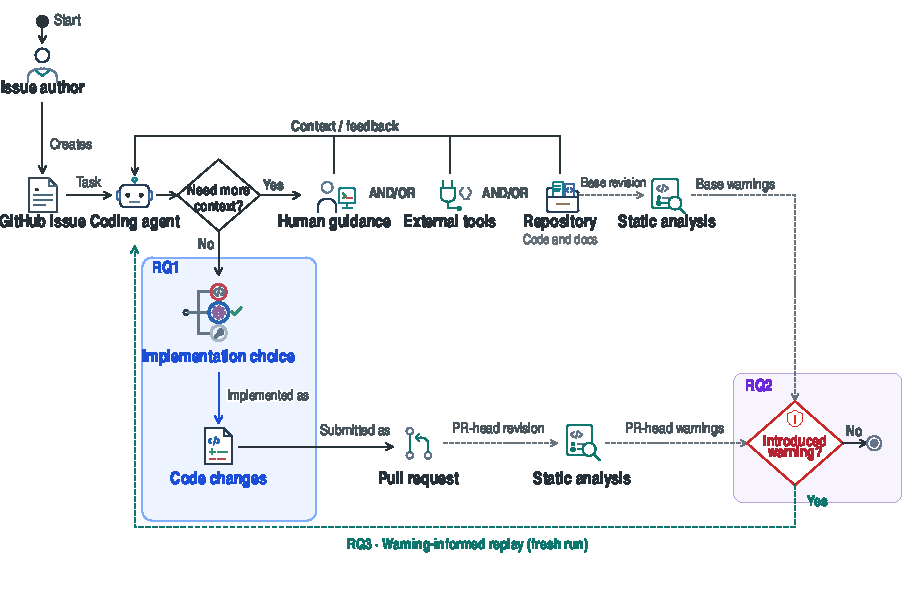
\includegraphics[width=\linewidth]{assets/figures/Fig1_Conceptual.pdf}
\caption{Workflow overview showing issue-driven implementation, possible context sources, base/head checks and warning-informed reimplementation. The RQ2 marker denotes the new-finding comparison used to define the matched groups, rather than the wording analysis itself. This is a conceptual workflow, not a verified execution trace.}
\Description{The workflow depicts an issue author, a coding agent, possible human, tool and repository context, implementation changes, a pull request, before-and-after security checks and warning-informed reimplementation.}
\label{fig:original-workflow}
\end{figure}

\begin{figure}[H]
\centering
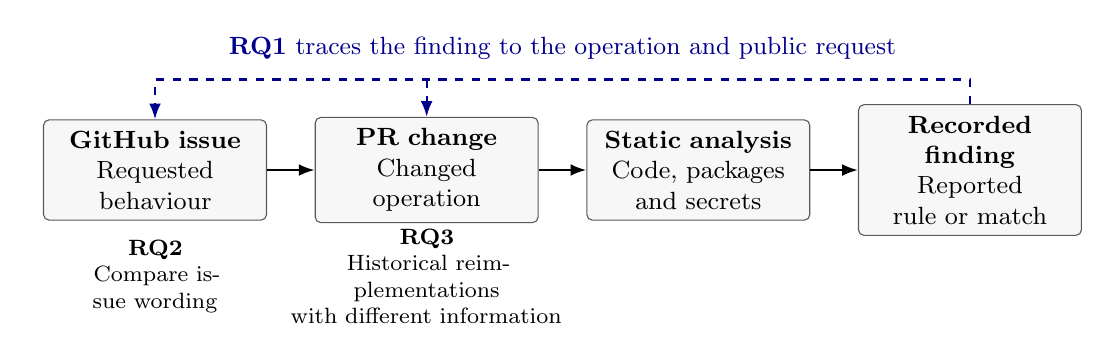
\begin{tikzpicture}[
  font=\small,>={Latex[length=2mm]},
  box/.style={draw=black!65,fill=black!3,rounded corners=2pt,align=center,text width=2.55cm,minimum height=1.05cm,inner sep=4pt},
  forward/.style={->,line width=.8pt},
  trace/.style={->,dashed,line width=.8pt,draw=blue!55!black}]
\node[box] (issue) at (0,0) {\textbf{GitHub issue}\\Requested behaviour};
\node[box] (change) at (3.45,0) {\textbf{PR change}\\Changed operation};
\node[box] (analysis) at (6.9,0) {\textbf{Static analysis}\\Code, packages\\and secrets};
\node[box] (finding) at (10.35,0) {\textbf{Recorded finding}\\Reported rule or match};
\draw[forward] (issue) -- (change);
\draw[forward] (change) -- (analysis);
\draw[forward] (analysis) -- (finding);
\draw[trace] (finding.north) -- (10.35,1.15) -- (0,1.15) -- (issue.north);
\draw[trace] (3.45,1.15) -- (change.north);
\node[font=\small,align=center,text=blue!55!black] at (5.175,1.55) {\textbf{RQ1} traces the finding to the operation and public request};
\node[font=\footnotesize,align=center,text width=3cm] at (0,-1.35) {\textbf{RQ2}\\Compare issue wording};
\node[font=\footnotesize,align=center,text width=3.6cm] at (3.45,-1.35) {\textbf{RQ3}\\Historical reimplementations\\with different information};
\end{tikzpicture}
\caption{The relationship examined in the study. Solid arrows show conceptual links, not verified instruction flow in an agent session. RQ1 relates a reported finding to the changed operation and the public issue. RQ2 compares issue wording, while RQ3 examines new implementations of selected historical tasks.}
\Description{A public issue, a changed PR operation, static analysis and a finding form the conceptual chain. Dashed arrows trace the finding back to the operation and issue. RQ2 examines issue wording and RQ3 historical reimplementations.}
\label{fig:overview}
\end{figure}


\Needspace{20\baselineskip}
\subsection{Research Questions}\label{sec:rqs}
\vspace{\baselineskip}

The study asks three questions of unequal weight. RQ1 provides the main evidence. If warnings concern techniques that issues leave open, two further questions follow: whether less specific issues are the ones linked to new findings (RQ2), and whether supplying the missing security information changes the implementation (RQ3).
\begin{itemize}
\item \textbf{RQ1.} How do recorded security findings in agent-associated pull requests relate to what their linked issues request?
\item \textbf{RQ2.} Does issue instruction specificity differ between issues linked to PRs with newly recorded findings and issues linked to matched PRs without new findings under comparable completed checks?
\item \textbf{RQ3.} In exploratory replays of historical tasks, how do the implementation and CodeQL findings differ between the original issue alone, the issue with its historical warning, and the issue with a security property derived from that warning?
\end{itemize}

\subsection{Contributions}

The main contribution is an empirical account, at the level of individual changed operations, of how recorded security findings relate to issue requirements in naturally occurring merged PRs. In an initial cohort of 122 instances, the analysis links 605 findings to 322 responsible changes and distinguishes changes that are Direct (implement requested behaviour) from changes that are Supporting (accompany it), as described in Sections~\ref{sec:attrib} and~\ref{sec:roles}. Source-linked cases then show requested functionality implemented through flagged techniques that the issues did not prescribe, and an extended analysis groups responsible changes into implementation choices and examines earlier public evidence for them (populations in Table~\ref{tab:population-guide}). Two secondary analyses, a matched comparison of issue wording and a set of retrospective replays, explore how guidance relates to recorded findings. The rest of the paper gives the background (Section~\ref{sec:background}), reviews related work and states the gap (Section~\ref{sec:related}), describes the study design and methods (Section~\ref{sec:methods}), reports the results by research question (Section~\ref{sec:results}), discusses them (Section~\ref{sec:discussion}), sets out the threats to validity (Section~\ref{sec:threats}) and concludes (Section~\ref{sec:conclusion}).

\section{Background}\label{sec:background}

\subsection{Tasks, Patches and Coding Agents}

GitHub issues record requested functionality, defects and discussion; PRs record proposed changes. Their links permit analysing a request alongside a patch, but do not prove that the public issue initiated, fully specified or dictated the implementation \cite{b5}. Coding agents may also use repository instructions, files and tool output absent from the public issue \cite{b20,b22}. \emph{Agent-associated} means that public PR metadata, branch patterns or issue/PR text indicate coding-agent involvement; a tool mention does not prove agent authorship, so the sample is not a census of autonomously written patches.

\subsection{Warnings, Advisories and Retained Findings}

CodeQL and Semgrep flag patterns in source code \cite{b44,b52}; OSV and Trivy report vulnerable dependencies \cite{b51,b50}, while Gitleaks identifies possible secrets \cite{b53}. CodeQL's query-based approach builds on QL, a language designed for querying program representations \cite{b44}. Throughout the paper, a \emph{finding} is one retained warning from any of these tools, whether it comes from static analysis, dependency inspection or secret detection, not a confirmed vulnerability. For RQ3, the recorded count is specifically the number of new CodeQL alerts in a generated patch.

A PR, and with it the linked issue, is \emph{finding-positive} when the recorded before/after comparison detects at least one new finding. A \emph{control} has no new findings under the applicable checks that completed successfully. Controls may still have older findings or lack results from other tools; neither label establishes exploitability or functional correctness.

\subsection{Task Relevance and Implementation Choice}

Four units recur throughout the paper. A \emph{finding} is a retained warning from static analysis, dependency inspection or secret detection, as defined above. A \emph{responsible change} is the code or dependency operation in the PR to which one or more findings are linked. A \emph{task role} describes how a responsible change relates to the requested behaviour, and is Direct (implements requested behaviour), Supporting (accompanies it) or Unclear. Related responsible changes within one linked issue--PR pair, called an \emph{instance}, are grouped into an \emph{implementation choice}, which describes an observable implementation technique and is neither a separate finding nor a verified private decision by an agent. Task role and technique are assessed separately. Suppose an issue asks for an @-mentioned file to be included in a prompt. Reading that file directly addresses the request, which is a matter of task role. Checking its metadata and then reading it by pathname is one particular technique for doing so, which the issue need not prescribe. Table~\ref{tab:m1} gives the classification rules for both.

\section{Related Work}\label{sec:related}

\subsection{Coding Agents and How They Are Judged}

SWE-bench evaluates software-repair patches against tests for 2,294 GitHub issues drawn from 12 Python repositories \cite{b9}. SWE-agent, AutoCodeRover and OpenHands provide repository-level interfaces for agents to inspect files, edit code and run tests \cite{b22,b25,b20}. Trae Agent studies test-time scaling for repository-level issue resolution by generating and selecting candidate solutions \cite{b47}. These systems and benchmarks primarily evaluate task completion; the present study instead examines the relationship between recorded security findings, the changes that produced them and the issue requirements.

\subsection{Crafted Issues and Untrusted Context}

Przymus et al. show that adversarial bug reports can lead automated repair agents to introduce attacker-aligned changes \cite{b16}. SWExploit constructs misleading issue reports intended to induce functionally correct but vulnerable patches \cite{b3}. AgentDojo and InjecAgent benchmark prompt injection through untrusted tool outputs and other external content; Liu et al. examine attacks against coding editors \cite{b6,b24,b12}. Related defences study detecting and removing injected instructions (PromptArmor) and applying program analysis to agent runtime traces (AgentArmor) \cite{b45,b46}. These experiments investigate adversarial instructions or runtime defences. This paper instead examines naturally occurring merged PRs without assuming that their linked issues are attacks.

\subsection{Agent Pull Requests and Issue Mining}

Public signals such as account identities, branch names and co-authorship metadata have been used to study coding-agent PRs at scale. Li et al. analyse agent participation in open-source development, while Watanabe et al. examine how agent-associated PRs are used and integrated on GitHub \cite{b11,b21}. The links between issues and PRs have their own structure and do not necessarily establish which public text initiated a change \cite{b5}. Prior issue research examines the requests made in open-source AI projects and the characteristics of beginner-friendly issues \cite{b23,b26}; RQ2 likewise characterises issue text, by instruction specificity. This study uses issue links and coding-agent indicators to select its cohort, then inspects the code behind recorded findings rather than treating a link as proof of the instructions received by an agent.

\subsection{Static-Analysis Warnings and Generated Code}

Static-analysis findings need interpretation. Johnson et al. report that developers' use of static-analysis tools is affected by false positives and how the warnings fit their workflow \cite{b33}. Pearce et al. assess the security of GitHub Copilot suggestions, showing why plausible code needs security assessment \cite{b35}.

Closer work examines complete patches. Sajadi et al. compare developer, LLM and agent patches on SWE-bench using CodeQL, Semgrep and Bandit. They also examine issue-level information, including code snippets, expected behaviour and reproduction steps \cite{b48}. Their analysis therefore already connects issue context with security outcomes. Rabbi et al. apply before/after Semgrep scans to 675 agent-associated PRs selected as security-related and examine weakness categories, review outcomes and rejection reasons \cite{b49}. The present study differs in selection and in unit of analysis. It selects merged, issue-linked JavaScript/\allowbreak TypeScript work without requiring a security-related description. Where those studies, as summarised here, relate findings to patches, issue-level information and PR outcomes, this study relates each finding to the specific changed operation and to what the issue required of it.

\subsection{Research Gap}

Existing studies evaluate task completion \cite{b9,b22}, investigate crafted attacks \cite{b3,b16}, characterise agent-associated PRs \cite{b11,b21}, and analyse security findings in generated patches or security-related PRs \cite{b48,b49}. Together they show that agent-associated changes can carry security findings and, in the case of Sajadi et al., that issue context can be connected with security outcomes \cite{b48}. Relative to the work summarised above, this study adds one step: identifying the changed operation behind each finding and comparing it with what the issue asked for, in naturally occurring merged pull requests. A static analysis tool reports a warning at a location, but that location need not be code the PR changed. A data-flow warning can point to a statement that predates the PR, and a dependency advisory names a package version rather than an edit. The operation responsible therefore has to be identified from the PR diff together with the tool output, and only then can it be compared with what the issue asked for. Without this identification and comparison, a finding in code that fulfils the request cannot be distinguished from one in an accompanying test or a regenerated lockfile, and a technique that the issue prescribed cannot be distinguished from one that it left open. In naturally occurring work, unlike in constructed attacks, neither the responsible operation nor the intended effect of the issue is known in advance. The matched comparison and retrospective replays provide supporting, exploratory evidence about issue specificity and additional security information. RQ2 follows the issue-level direction that Sajadi et al. examine, using instruction specificity.

\section{Study Design and Methods}\label{sec:methods}

I conducted an observational study of merged, agent-associated PRs linked to public GitHub issues in JavaScript and TypeScript repositories. The study selected issue--PR instances, compared security analysis results before and after each PR, linked new findings to responsible changes (RQ1), compared issue wording with matched controls (RQ2), and examined retrospective warning-informed replays (RQ3). Figure~\ref{fig:overview} shows the conceptual relationship between the public request, implementation and finding; Table~\ref{tab:population-guide} identifies the populations used in each analysis.

\Needspace{6\baselineskip}
The analysis uses the units defined in the Background (finding, responsible change, task role and implementation choice), with one linked issue--PR pair as an \emph{instance}. RQ2 analyses matched instance pairs, and RQ3 analyses generated patches for selected historical tasks.

Figure~\ref{fig:study-overview} gives the study at a glance. Of the 3,809 selected instances, 192 have newly recorded findings under the completed applicable checks, which cover static analysis of code, dependency inspection and secret detection. RQ1 traces those findings to changed operations, RQ2 compares matched pairs, and RQ3 replays selected historical tasks.

\begin{figure}[H]
\centering
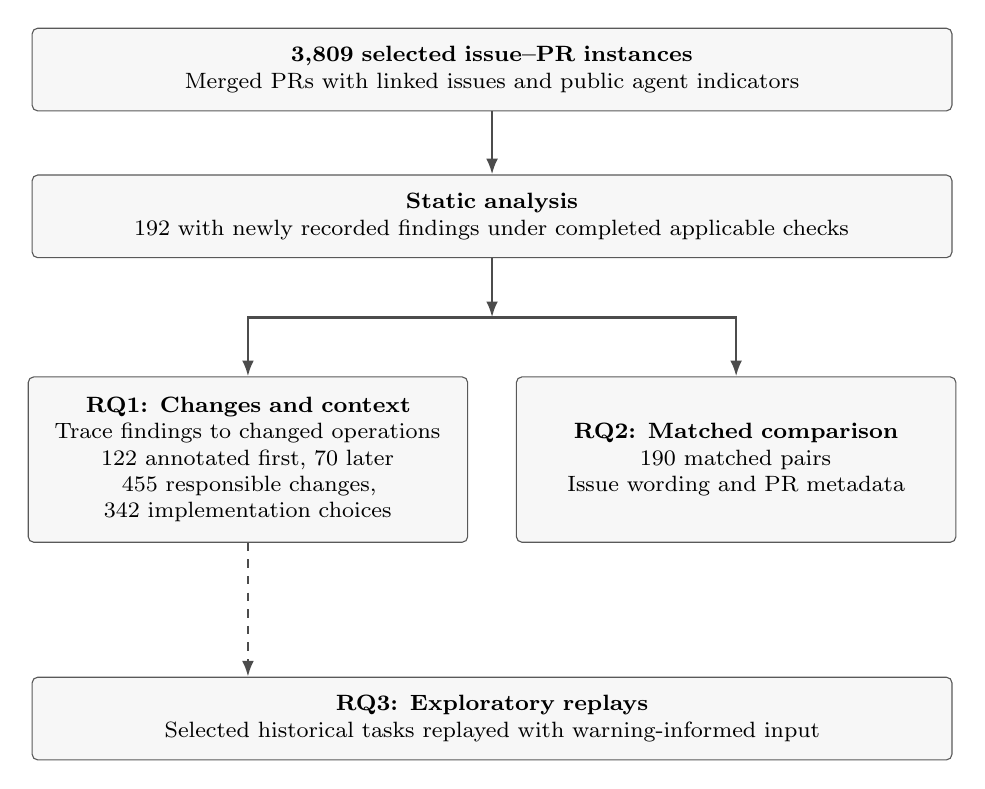
\begin{tikzpicture}[
  font=\footnotesize,>={Latex[length=2mm]},
  wide/.style={draw=black!65,fill=black!3,rounded corners=2pt,align=center,text width=11.4cm,minimum height=1.05cm,inner sep=4pt},
  panel/.style={draw=black!65,fill=black!3,rounded corners=2pt,align=center,text width=5.3cm,minimum height=2.1cm,inner sep=4pt},
  link/.style={->,line width=.9pt,draw=black!70},
  weak/.style={->,dashed,line width=.9pt,draw=black!70}]
  \node[wide] (cohort) {\textbf{3,809 selected issue--PR instances}\\ Merged PRs with linked issues and public agent indicators};
  \node[wide,below=8mm of cohort] (checks) {\textbf{Static analysis}\\ 192 with newly recorded findings under completed applicable checks};
  \node[panel,anchor=north] (rq1) at ($(checks.south)+(-3.1cm,-1.5cm)$) {\textbf{RQ1: Changes and context}\\ Trace findings to changed operations\\ 122 annotated first, 70 later\\ 455 responsible changes,\\ 342 implementation choices};
  \node[panel,anchor=north] (rq2) at ($(checks.south)+(3.1cm,-1.5cm)$) {\textbf{RQ2: Matched comparison}\\ 190 matched pairs\\ Issue wording and PR metadata};
  \node[wide,anchor=north] (rq3) at ($(rq1.south)!0.5!(rq2.south)+(0,-1.7cm)$) {\textbf{RQ3: Exploratory replays}\\ Selected historical tasks replayed with warning-informed input};
  \coordinate (fork) at ($(checks.south)+(0,-0.75cm)$);
  \draw[link] (cohort) -- (checks);
  \draw[link] (checks.south) -- (fork);
  \draw[link] (fork) -| (rq1.north);
  \draw[link] (fork) -| (rq2.north);
  \draw[weak] (rq1.south) -- (rq1.south |- rq3.north);
\end{tikzpicture}
\caption{Study overview: population, RQ1 attribution, RQ2 matched comparison and RQ3 selected replays. The instances with newly recorded findings come from all completed applicable checks, that is, static analysis of code, dependency inspection and secret detection. Solid arrows show which instances feed each analysis and carry no causal meaning; RQ2 additionally draws its controls from instances without new findings. The dashed arrow marks that replay tasks derive from historical instances with CodeQL warnings; the 14 tasks are a selected set, and RQ3 does not use the RQ2 pairs.}
\Description{A study overview: 3,809 selected instances lead to static analysis and 192 instances with findings, which feed RQ1 (changes and context) and RQ2 (matched comparison); a dashed arrow leads from RQ1 to RQ3 (exploratory replays).}
\label{fig:study-overview}
\end{figure}

\begin{table}[H]
\caption{Study populations and units. The subsets overlap and must not be added together.}
\label{tab:population-guide}
\footnotesize\renewcommand{\arraystretch}{1.10}
\begin{tabularx}{\linewidth}{@{}L{2.65cm}L{2.2cm}Y@{}}
\toprule
\textbf{Population} & \textbf{Size} & \textbf{Use in the paper}\\
\midrule
Full corpus & 3,809 instances & Merged, issue-linked PRs; security analysis comparisons.\\
Finding-positive & 192 instances & At least one newly recorded finding.\\
Initial annotations & 122 instances & 605 findings linked to 322 responsible changes.\\
Extended mapped set & 191 instances & 455 responsible changes grouped into 342 implementation choices; one positive has no mapped change.\\
Matched comparison & 190 pairs & One positive and one control per RQ2 pair.\\
O/W/P replays & 14 tasks & 12 complete sets of three generated patches.\\
\bottomrule
\end{tabularx}
\end{table}



\subsection{Population and Selection}

I searched GitHub for merged PRs linked to issues (qualifiers \texttt{is:pr}, \texttt{is:merged}, \texttt{linked:issue}) in non-archived JavaScript/\allowbreak TypeScript repositories with at least 100 stars, merged between 1 November 2025 and 11 August 2026. JavaScript and TypeScript match the CodeQL and Semgrep rule sets applied, the start date keeps the sample recent, and the star cutoff limits the sample by repository popularity. The snapshot contains 3,809 distinct issue--PR instances in 723 repositories (609 JavaScript, 3,200 TypeScript; selection criteria and cohort characteristics in Table~\ref{tab:cohort}). Agent indicators include PR authorship or metadata, branch and description markers, and weaker issue-side references to Codex, Copilot, Cursor, Claude or Devin; for 236 instances the only association is an issue-side marker, not PR-side evidence. The 100-star threshold is a sampling filter rather than a quality measure. Stars and language are snapshot metadata, not values reconstructed at each merge date.

\subsection{Detecting and Retaining Introduced Findings}

The pipeline records whether each security analysis tool applies, whether it ran successfully and what it reported (Table~\ref{tab:scanners}). CodeQL and Semgrep findings are counted as introduced when the archived comparison reports them after, but not before, a PR. In the initial annotation cohort, described next, retained source-code findings also have a primary or data-flow location on a PR-added line. These are \emph{introduced findings}, not independently established new vulnerabilities. A changed data-flow path may affect an existing flagged statement (Table~\ref{tab:scanners}).

Of the 3,809 instances, 192 had newly recorded findings. The remaining 3,617 had none under their completed applicable checks; this does not imply that every tool ran. The initial annotation cohort of 122 instances, which is not a random sample, was retained from 138 apparent positives identified in an August 2026 snapshot, after the exclusion of four with no introduced finding under corrected merge-base checks and twelve that lost all findings during dependency validation. Tables and the supplement call it the original cohort, and I use both names. A further 70 were added in a later annotation tranche. One positive had no exactly mapped change, leaving the 191-instance mapped set in Table~\ref{tab:population-guide}. The initial cohort's 605 findings and 322 responsible changes should not be confused with the 455 changes in the extended mapped set.

Dependency results received an additional merge-base verification in the initial annotation cohort. Package/version records were compared at the PR's true merge base and head, which is the dependency validation that excluded the twelve instances above. Most candidate package/version transitions proved to be already present at the merge base and were not attributed to the PR (Section~\ref{sec:s2}). Comparable verification is not established for the 70 later positives, so I do not generalise the stronger verification claim to them.

\subsection{Removing Duplicates and Linking Findings to Changes}\label{sec:attrib}

A finding and its responsible change are different. Several responsible changes can also belong to one implementation choice: in T3Code, two CodeQL rules flag two changes that are parts of one regular-expression strategy (Section~\ref{sec:s3}). Repeated records of the same finding within an instance were merged, while distinct rules and advisories were kept separate. This yielded 605 findings from 832 raw tool references in the 122-instance cohort. For source-code warnings the comparison used reported rules and locations, changed hunks and available pre-change code. For dependency findings it used declared or resolved versions before and after the PR. A reported file location alone did not establish the responsible operation; Table~\ref{tab:mapping} gives the mapping basis of every finding.

I used model-assisted annotation to propose the code, configuration or dependency change responsible for each retained finding. The model received the finding, tool output and PR diff, but not the issue text or PR description. A candidate link was retained only when the record identified a changed file, a line or diff hunk, and an explanation of how that change accounts for the finding. Each retained link therefore has recorded supporting evidence but was not independently human-verified.

For 142 dependency findings in the original cohort, recorded merge-base verification supports the package/version attribution; 36 of these links were resolved during that verification. The underlying dependency verification records and counts are given in Section~\ref{sec:s2}.

The recorded annotation model was GPT-5.6 Sol with medium reasoning effort. Because one responsible change can account for multiple findings, the two counts are reported separately. Independent validation limits are discussed in Section~\ref{sec:threats}. Subsequent task-role coding compares the mapped change with the issue's requested goals; it does not independently revalidate the finding-to-change link (Section~\ref{sec:roles}). Case evidence is presented in Sections~\ref{sec:s3} and~\ref{sec:s6}.

Figure~\ref{fig:rq1-method} shows how retained findings are linked to responsible changes, assigned task roles and grouped into implementation choices. Model-assisted grouping of the 455 changes yields 342 choices within instances. Each choice is classified as publicly prescribed, mechanically generated, selected among alternatives or unresolved, using only evidence available before the change (Table~\ref{tab:m1}). Choices made among alternatives are further described using the explanation tiers T1 to T5 in Table~\ref{tab:rules-full}; these tiers are a different thing from the classification code T, which marks a choice produced mechanically by a tool.

\begin{figure}[!tbp]
\centering
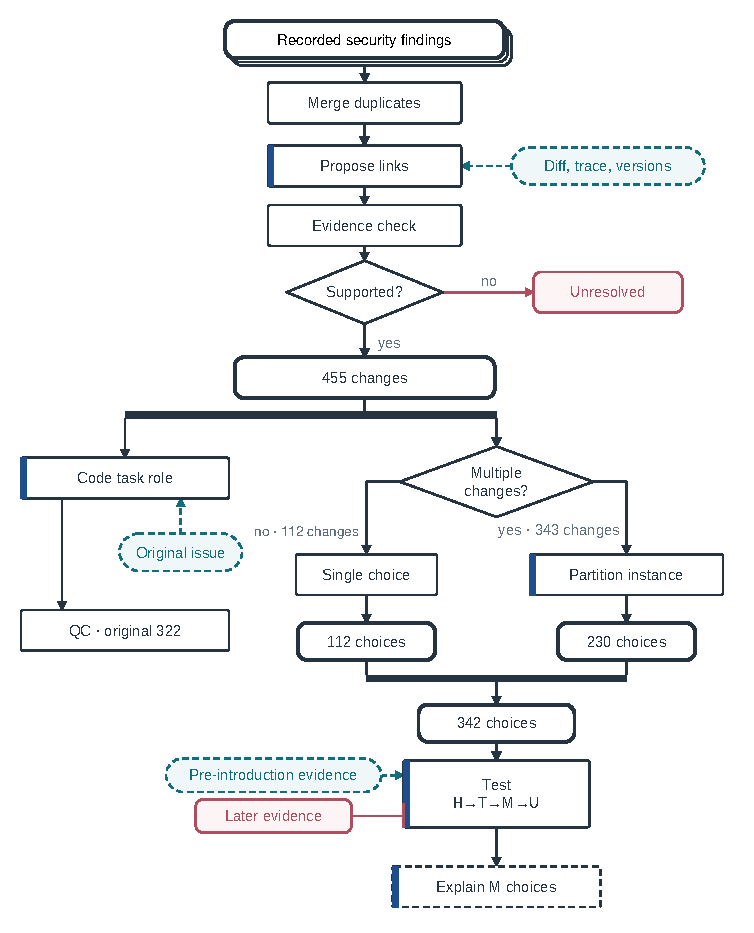
\includegraphics[width=0.9\textwidth]{assets/figures/RQ1_Methodology.pdf}
\caption{From findings to responsible changes and implementation choices. Blue bars mark model-assisted steps; teal callouts identify admissible evidence, and red marks unsupported links or later evidence excluded from origin coding. Dark outlines show retained counts. The first yes/no decision tests link support; the second distinguishes changes grouped into choices. The dashed final box denotes explanation tiers for $M$ choices. Retained links require a changed file, line or hunk and a supporting explanation (Section~\ref{sec:attrib}).}
\Description{Findings are deduplicated and linked to changed operations using code evidence. Operations receive task roles and are grouped into implementation choices, which are classified using earlier public evidence.}
\label{fig:rq1-method}
\end{figure}

In Case~3 (Section~\ref{sec:rq1-open}), for example, CodeQL's file-system-race warning is the finding and the PR's added check-then-read sequence is the responsible change.

\subsection{Task Role, Affected Files and Earlier Public Evidence}\label{sec:roles}

I used model-assisted coding to assign task roles by comparing a factual operation summary with the issue's requested goals (Table~\ref{tab:m1}). The labels (Direct, Supporting, Unclear) describe the operation's role, not whether its technique was publicly prescribed or who chose it. The annotations also record the finding family and the affected file type, distinguishing production source, tests or fixtures, documentation or examples, dependency manifests and generated lockfiles. File type refers to the finding's reported location, which need not be the file containing the mapped change. A pattern in a test or README does not imply the exposure of the same pattern in deployed code.

For the original 322 changes, an initial model-assisted pass assigned task roles using the previously fixed issue request and the change evidence, without PR-description text or complete finding records. A subsequent source-assisted quality-control pass revised 11 roles (seven Direct to Supporting and four Supporting to Direct); the original annotation records retain the earlier and final labels and case-specific reasons. The 133 later changes also have model-assisted roles.

The extended mapped set contains 455 responsible changes grouped into 342 implementation choices. Model-assisted coding then distinguishes techniques prescribed in earlier public evidence, changes produced mechanically by tools or dependency resolution, and techniques selected among plausible alternatives. Unresolved is allowed where evidence is insufficient (Table~\ref{tab:m1}). For choices made among alternatives, a separate classification describes the strength of any earlier public precedent. Three comparisons bear on these labels, and they are distinct. The first is between two isolated model passes, which agreed on how the choice arose (H, T, M or U) for 337 of 342 choices (98.5\%, $\kappa=0.97$). They agreed on the explanation tier for only 88 of 232 choices selected among alternatives ($\kappa=0.09$), so the tier labels are the least reliable output. Both passes classed 232 choices as selected among alternatives; the primary classification, which includes my final selections, contains 233. The second compares the primary classification, whose counts this paper reports, with an earlier classification version (Table~\ref{tab:routes}). The third is my own selection of final labels for a set of disputed choices, described next. For a set of 50 implementation choices, the earlier labels disagreed on 42, in 40 of them on the explanation tier only. After reviewing explanatory material and recorded source comparisons prepared with model assistance, I selected a final classification and tier for 41 of these disputed choices and left one undecided. None of the 41 changed classification (H, T, M or U); 17 changed tier, 14 of them toward stronger precedent. Tier assignment depends on interpreting sparse pre-change evidence, so I treat the tier labels as indicative, and no main-text claim depends on them. The eight remaining choices, on which all earlier labels agreed, were not re-labelled. This was a post-hoc selection among model-presented evidence, not blinded or independent coding.

I assessed earlier public evidence against the recorded time of the change. Some linked issues were created after their PRs. In the original 122 instances, 4 PRs were opened before their linked issue and 15 more within 10 minutes after it; Section~\ref{sec:threats} states what a Direct label can show. These are PR creation times, not the time the implementing code first appeared, and the public issue may omit private user or agent messages. A technique's first appearance in the patch, or the absence of an earlier public example, does not establish that the agent invented it.

The Chaibuilder case (Section~\ref{sec:s3}) shows how the units fit together. The issue asked for the Next.js framework to move from Tailwind CSS v4 to v3. The PR changed the \texttt{tailwindcss} dependency constraint and refreshed the lockfile, and the dependency checks then recorded one dependency downgrade and several advisories on lockfile entries. These are the findings. They map to seven responsible changes, namely the edited constraint and six lockfile entries. The constraint change is Direct, because it implements the requested move to v3, and it forms one implementation choice selected among alternatives, because the issue asked for v3 without saying how the constraint should be written. The six lockfile entries are Supporting and are classified as mechanically produced (code T in Table~\ref{tab:m1}).

\begin{table}[!tbp]
\caption{RQ1 classification rules and their limits. Task role is decided per responsible change; how it arose per grouped choice.}
\label{tab:m1}
\fontsize{8}{10}\selectfont\renewcommand{\arraystretch}{1.1}
\begin{tabularx}{\linewidth}{@{}L{2.5cm}YY@{}}
\toprule
\textbf{Category} & \textbf{Decision rule} & \textbf{Interpretation}\\
\midrule
\multicolumn{3}{@{}l}{\textit{Task role (per responsible change)}}\\
\textbf{Direct} & Implements a substantive goal of the public issue. & The issue need not prescribe the mechanism.\\
\textbf{Supporting} & Enables or accompanies the requested work rather than fulfilling it, including incidental implementation choices the issue did not request. & Role is not inferred from file type alone.\\
\textbf{Unclear} & Evidence cannot establish the task relation. & Uncertainty is retained, not forced into a binary.\\[2pt]
\multicolumn{3}{@{}l}{\textit{How the implementation choice arose (per grouped choice)}}\\
\textbf{H --- prescribed} & Pre-introduction public evidence specifically fixes the mechanism. & A broad goal or later evidence is insufficient.\\
\textbf{T --- mechanical} & Dependency resolution, generated artifacts or tooling produce the choice. & Not evidence of discretionary choice.\\
\textbf{M --- selected among alternatives} & One implementable technique was used although public evidence did not require it and plausible alternatives exist. & A known precedent may explain the choice; its source is not established.\\
\textbf{U --- unresolved} & Evidence cannot separate H, T and M. & Missing evidence is not proof of choice.\\
\midrule
\textbf{Earlier public evidence} & For M choices, note any reused code, repository precedent, stated contract or contextual support. & Its availability does not show that the contributor saw it.\\
\bottomrule
\end{tabularx}
\end{table}

\subsection{Matched Controls and Issue Coding}\label{sec:rq2-design}

RQ2 compares how issues are worded in finding-positive instances and in matched controls with no newly recorded finding under the checks that applied and completed. Controls may carry older findings, and not every tool ran on each instance. The recorded matching procedure paired each PR with new findings with at most one control PR without recorded new findings. Issue-wording annotations were joined after matching. Eligible controls had to cover the positive instance's completed applicable checks, fall within 90 days of its PR creation date and have changed-line and changed-file counts within a factor of about four. Cross-repository controls required exactly the same set of completed checks. The matcher preferred controls from the same repository. Issue wording, review variables and agent identity were not additional matching criteria (Figure~\ref{fig:rq2-method}; protocol in Section~\ref{sec:s5}). Of the 192 positives, 190 were matched (115 same-repository, 75 cross-repository; Table~\ref{tab:rq2-diag}). The analysis used the existing matching records without rerunning the procedure. Matching does not equate the tasks or randomise the wording.

Each issue received one of three wording labels, Problem only, Suggests solution or Explicit instruction. They describe the specificity of wording, not whether a security requirement was stated or the exact technique prescribed. An Explicit instruction label therefore does not imply an H classification for the implementation choice. Positive issues and controls were coded in separate passes; the control pass withheld security analysis outcomes and pair identities. Because cross-pass agreement was not measured, some of the wording difference could reflect coding differences (Section~\ref{sec:threats}). The 121 original-cohort pairs and the 115 same-repository pairs are nested sensitivity subsets, not independent replications. The matched pair is the unit of analysis. I used a paired Stuart--Maxwell test to compare the three issue-wording categories. The primary test was recomputed from the reported contingency table (Table~\ref{tab:rq2}); the Holm adjustment within a family of nine comparisons and the secondary comparisons are taken from the archived analysis (Section~\ref{sec:s5}).

\subsection{Retrospective and Information-Guided Replays}\label{sec:rq3-design}

The RQ3 replays are a retrospective diagnostic, separate from the RQ2 pairs (definitions and protocols in Section~\ref{sec:s6}, inputs in Table~\ref{tab:m2} and design in Figure~\ref{fig:rq3-method}). Fourteen historical tasks were assigned three input conditions. O supplies the original issue, W adds its historical CodeQL warning, and P adds a security property derived from that warning without naming the rule. W and P were constructed using historical warnings. The experiment therefore does not establish whether equivalent guidance could be identified before implementing a new task. Of 42 intended outputs, 40 are retained (12 O, 14 W and 14 P), giving 12 complete O/W/P triples; the two missing O outputs are not imputed. One output was retained per available task and input condition. The records link these outputs to scan results and baseline identifiers, but do not establish comparable, independent model sessions or functional equivalence across conditions. The tasks were selected for prior CodeQL warnings rather than sampled randomly.

Section~\ref{sec:s6} explains why a separate, incompletely documented pilot is excluded from the replay comparisons.

New CodeQL alerts, including those sharing the historical rule, are reported for the 12 complete triples against their recorded baselines (Table~\ref{tab:replays}). 

\section{Results}\label{sec:results}

The results address RQ1 first and then turn to issue wording (RQ2) and replay outcomes (RQ3). The main observations are numbered Observation~1 to Observation~8, and each subsection closes with a direct answer to its research question.

\subsection{RQ1 --- Findings and the Changes Behind Them}\label{sec:rq1-roles}

\emph{Observation 1.} Findings and responsible changes are different quantities. In the initial annotation cohort of 122 instances, 605 findings were linked to 322 responsible changes, because a single change can produce several findings. The \href{https://github.com/Pimzino/spec-workflow-mcp/pull/173}{spec-workflow-mcp PR} is the clearest example. It refreshed a lockfile while addressing a path-translation problem, and its 131 dependency-related findings map to 36 changes, each a package version absent at the merge base and present at the head. Figure~\ref{fig:concentration} shows how far a handful of such instances dominate the finding totals; detailed counts are in Table~\ref{tab:concentration}. The gap between findings and changes persists when findings linked only through a data-flow location and instances with only issue-side agent markers are excluded (Section~\ref{sec:s4}).

\begin{figure}[H]
\centering
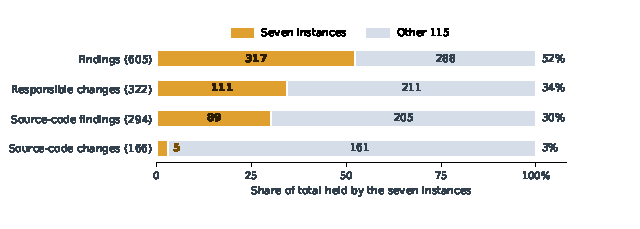
\includegraphics[width=0.7\linewidth]{assets/figures/Fig5_Concentration.pdf}
\caption{A few instances hold many findings but almost none of the source-code changes. Each bar splits one total between the seven instances with the most findings and the other 115 in the original cohort. The seven hold 52\% of all findings but only 3\% of source-code responsible changes. Counts for the seven are the totals minus the excluded-seven counts in Table~\ref{tab:concentration}.}
\Description{The seven instances with the most findings account for more than half of findings but only five of 166 source-code responsible changes. Dependency and data-flow reports account for much of the concentration.}
\label{fig:concentration}
\end{figure}

Seven instances account for more than half of the findings but only five of the 166 mapped source-code changes, and much of this concentration reflects dependency findings and repeated data-flow warnings. Ranking PRs by warning count would therefore foreground a few dependency updates and test operations rather than the source-code changes behind the other warnings.

\emph{Observation 2.} The relationship to the requested task varies by finding family (Table~\ref{tab:role}). Task role is assigned to each responsible change and is not inferred from the number of warnings it produced. Most of the 322 changes were Supporting (228). Dependency-related changes were almost all Supporting, as in spec-workflow-mcp, where every change from the lockfile refresh was Supporting. The source-code changes in this cohort, by contrast, divided evenly, with 82 Direct and 82 Supporting.

\begin{table}[!tbp]
\caption{Findings and responsible changes by finding family and task role: Direct (implements requested behaviour), Supporting (accompanies it) or Unclear.}
\label{tab:role}
\small
\begin{tabular}{@{}l>{\columncolor{unitshade}}r@{\hspace{10pt}}rrrr@{}}
\toprule
& \multicolumn{1}{>{\columncolor{unitshade}}c}{\textbf{Findings}} & \multicolumn{4}{c}{\textbf{Responsible changes (task role)}}\\
\cmidrule(l{2pt}r{2pt}){2-2}\cmidrule(l){3-6}
\textbf{Finding family} & \multicolumn{1}{>{\columncolor{unitshade}}r}{Reported} & \textbf{Total} & Direct & Supporting & Unclear\\
\midrule
Source-code warnings & 294 & \textbf{166} & 82 & 82 & 2\\
Dependency advisories and downgrades & 290 & \textbf{137} & 4 & 132 & 1\\
Secret-like findings & 18 & \textbf{16} & 3 & 13 & 0\\
Other dependency-version changes & 3 & \textbf{3} & 2 & 1 & 0\\
\midrule
Total & 605 & \textbf{322} & 91 & 228 & 3\\
\bottomrule
\end{tabular}
\par\smallskip\raggedright\footnotesize Original 122 finding-positive instances. A finding is one deduplicated tool report; a responsible change is the changed operation to which one or more findings were mapped, and task role is coded per responsible change. Not the extended 455-change population (Section~\ref{sec:s4}).
\end{table}

The even split between Direct and Supporting source-code changes describes the initial cohort, not a stable population-level balance. Excluding instances with only issue-side agent markers leaves 66 Direct, 79 Supporting and two Unclear changes (Section~\ref{sec:s4}). Under either count, similar numbers of source-code changes in this cohort implemented requested functionality and accompanied it, so a source-code warning alone does not tell a reviewer which kind of change it concerns.

\emph{Observation 3.} Where a warning is reported affects what it means. The location a tool reports need not identify the responsible PR change. In the original cohort, many source-code findings were linked through a data-flow or related location, not a primary location on a PR-added line (Table~\ref{tab:mapping}). In the GSD shutdown and recovery tests, for example, one added test operation in each PR accounted for many warnings reported in other files (Section~\ref{sec:s3}; location-mapping and sensitivity counts in Section~\ref{sec:s4}).

The affected file type matters as well. In Paperclip, file-system warnings arose in added regression tests; in dot-ai, a Gitleaks finding concerned a token placeholder in documentation. Both lie outside deployed source (source-linked records in Section~\ref{sec:s3}). Figure~\ref{fig:scanner} shows task-role classifications by reporting tool in the extended mapped set; its file-type panel retains the archived labelling of the dot-ai README as production source, a known misclassification noted in Section~\ref{sec:s3}. A warning may therefore need a different reading depending on the file it flags.

\subsection{RQ1 --- Requested Behaviour and Implementation Choices}\label{sec:rq1-open}

\emph{Observation 4.} Changes that directly implement a request can still use security-relevant techniques that the issue did not specify. A Direct role says that an operation implements what the issue asked for; it does not say that the issue chose how. Three cases make this difference concrete. In each, the requested functionality was delivered through a technique that the issue left unspecified, and a plausible alternative can be identified. The cases are explanatory examples, not a prevalence sample. Each card gives the request, the implemented operation, the resulting warning and an alternative approach; additional source-linked case evidence is provided in Section~\ref{sec:s3}.

\begin{casefile}{\textbf{Case 1 --- Spotify login verifier}\ \ {\scriptsize\texttt{ZHANGTIANYAO1/\allowbreak teamspeak-music-bot}}}{\href{https://github.com/ZHANGTIANYAO1/teamspeak-music-bot/issues/112}{Issue \#112}\ \ \href{https://github.com/ZHANGTIANYAO1/teamspeak-music-bot/pull/118}{PR \#118}}
\crow{Request}{Add Spotify as an audio source next to existing music services. The issue suggests a solution but says nothing about how the login verifier is built.}
\crow{What the PR did}{Builds the verifier by turning each random byte into a character with a remainder operation over a 66-character alphabet. 256 is not a multiple of 66, so some characters are slightly more likely.}
\crow{Warning}{CodeQL reports biased random values in a cryptographic setting.}
\crow{Reading}{The change implements the requested Spotify service and is classified as Direct, but the issue did not prescribe how to generate the verifier. The character distribution is non-uniform; exploitability was not assessed.}
\crow{Alternative}{The pre-PR repository already used \texttt{randomBytes(32).toString("base64url")} for session tokens in \href{https://github.com/ZHANGTIANYAO1/teamspeak-music-bot/blob/f8743a904f50a065c9fcf5139e46005b5fff2e46/src/data/sessions.ts\#L56}{\texttt{src/data/sessions.ts:56}}. This is a local example of random-token encoding without modulo reduction, but it was not evaluated as a drop-in replacement for the Spotify verifier. RFC 7636 describes this encoding method for generating a PKCE verifier \cite{b39}.}
\end{casefile}

\begin{casefile}{\textbf{Case 2 --- GSD tool-call repair}\ \ {\scriptsize\texttt{gsd-build/\allowbreak gsd-2}}}{\href{https://github.com/gsd-build/gsd-2/issues/2660}{Issue \#2660}\ \ \href{https://github.com/gsd-build/gsd-2/pull/3090}{PR \#3090}}
\crow{Request}{Milestone completion fails when the model writes YAML-style bullet lists into JSON tool arguments. The issue suggests making the JSON format clearer in prompts, templates or schema hints.}
\crow{What the PR did}{For the final tool-call arguments, the PR attempts strict parsing, uses a regular expression to repair bullet lists if that fails, and can fall back to a streaming parser. Other streaming paths are not assumed to follow this exact sequence.}
\crow{Warning}{CodeQL reports a regular expression that can take polynomial time on crafted input.}
\crow{Reading}{The runtime repair addresses the reported parsing failure (Direct). A regular-expression repair was not among the remedies the issue suggested.}
\crow{Alternative}{The remedies the issue itself named, or a repair that scans the text once without a backtracking pattern. The first is observed in the issue, the second is general practice.}
\end{casefile}

\begin{casefile}{\textbf{Case 3 --- Grok CLI file mentions}\ \ {\scriptsize\texttt{superagent-ai/\allowbreak grok-cli}}}{\href{https://github.com/superagent-ai/grok-cli/issues/235}{Issue \#235}\ \ \href{https://github.com/superagent-ai/grok-cli/pull/236}{PR \#236}}
\crow{Request}{Load files referenced with @-mentions into the prompt (Explicit instruction).}
\crow{What the PR did}{Looks up the path\textquotesingle s metadata and checks it is not a directory, then reads the file in a separate step. The file can change in between.}
\crow{Warning}{CodeQL reports a potential file-system race between checking and reading a path.}
\crow{Reading}{Direct. The issue did not prescribe a check-then-read sequence.}
\crow{Alternative}{Open the file once and read through that handle. A replay on a different file-access task generated a similar pattern (Section~\ref{sec:rq3-res}); this does not establish what the Grok CLI implementer considered.}
\end{casefile}



The Grok CLI issue was coded as an Explicit instruction, yet it left the file-access sequence open, so the specificity label does not mean that the technique was prescribed. Across the three cases, the techniques are unrelated (character selection, text repair and file access), and so are the grounds for regarding each as open: a local precedent in the Spotify repository, remedies named in the GSD issue itself, and a single-handle access pattern for Grok CLI. Four further cases (Neo.mjs, T3Code, KIRI, Paperclip; Section~\ref{sec:s3}) show related distinctions. The Chaibuilder case, worked through in Section~\ref{sec:roles}, shows the same separation of task role and technique for a dependency change; the Supporting classification of its six lockfile entries does not establish that the downgrade necessarily produced each entry. In the three main cases, the warning points at a decision the issue left open, not at the requested behaviour as such.

\emph{Observation 5.} Few of the 342 implementation choices were publicly prescribed. The extended analysis asks, for every grouped choice, whether public evidence prescribed the technique. In the primary classification, 6 choices were publicly prescribed, 103 were mechanically generated and 233 were selected among alternatives (Table~\ref{tab:routes}). These labels are model-assisted, and the comparisons in Section~\ref{sec:roles} bear on them. The two isolated model passes agreed on 337 of 342 classifications. Separately, 43 choices differ between the primary classification and an earlier classification version (Section~\ref{sec:s4}). Public prescription is rare in both classification versions (Table~\ref{tab:routes}), whereas individual labels are less stable than the totals, so I treat the remaining counts as support for the cases rather than as frequency estimates. In nearly all of these implementation choices, the technique was thus not publicly prescribed before the change.

RQ1 answer: In the original 122-instance cohort, most warning-associated changes supported the requested work (228 of 322) and fewer implemented it directly (91), while the examined cases and the classification of implementation choices in the extended set indicate that public evidence rarely prescribed the technique a flagged change used.

\subsection{RQ2 --- Issue Specificity in Matched Instances}\label{sec:rq2-res}

\emph{Observation 6.} Explicit implementation instructions were less common in issues linked to new findings. They appeared in 63.7\% of finding-positive issues and 77.9\% of matched controls. The controls thus had a 14.2-percentage-point higher proportion of explicit instructions than the finding-positive issues (approximate 95\% confidence interval 5.6--22.8 percentage points, a paired Wald interval computed from the discordant pairs). The paired comparison across all three wording categories gave a Holm-adjusted $p=0.00468$ (Table~\ref{tab:rq2}). Finding-positive issues more often suggested a solution without giving explicit instructions (33 versus 9), while Problem only issues were similarly frequent in both groups. The wording labels measure general implementation specificity, not security guidance, and the two groups were coded in separate passes. The difference has the same direction in the same-repository and original-cohort subsets (Section~\ref{sec:s5}). PR goals were also less often aligned with the issue in the finding-positive group (160 versus 183 of 190), a difference that weakens within repositories (Section~\ref{sec:s5}). Figure~\ref{fig:rq2-results} shows the paired differences in explicitness and goal alignment by task type. In this matched sample, less explicit issues and new findings occurred together.

\begin{table}[H]
\caption{Issue wording in 190 matched pairs. Rows give finding-positive issues and columns their matched controls with no newly recorded findings under completed applicable checks.}
\label{tab:rq2}
\small
\begin{tabular}{@{}lrrrr@{}}
\toprule
& \multicolumn{3}{c}{\textbf{Control issue wording}} & \\
\cmidrule(lr){2-4}
\textbf{Positive issue} & Explicit instruction & Problem only & Suggests solution & Total\\
\midrule
Explicit instruction & 98 & 15 & 8 & 121\\
Problem only & 25 & 10 & 1 & 36\\
Suggests solution & 25 & 8 & 0 & 33\\
\midrule
Total & 148 & 33 & 9 & 190\\
\bottomrule
\end{tabular}
\par\smallskip\raggedright\footnotesize Positive labels were fixed in earlier annotation stages; control labels were produced later from blinded packets. Stuart--Maxwell $\chi^2(2)=15.12$, $p=0.00052$ ($p_{\mathrm{Holm}}=0.00468$). Matching diagnostics and subset results are in Section~\ref{sec:s5}.
\end{table}

The GSD tool-call case (Case~2) gives an example of the labels. Its finding-positive \href{https://github.com/gsd-build/gsd-2/issues/2660}{issue} suggested prompt, template or schema remedies and was classified as suggesting a solution. Its same-repository control, \href{https://github.com/gsd-build/gsd-2/issues/2545}{issue \#2545}, specified expected operations and files for a queue command and was classified as an explicit instruction. The tasks differ, so this pair illustrates the coding categories rather than an effect of issue wording.

RQ2 answer: Issue instruction specificity differed as coded, with explicit instructions 14.2 percentage points less common in issues linked to new findings than in matched controls, an observational association about general specificity.

\subsection{RQ3 --- Alerts and Implementations in Replays}\label{sec:rq3-res}

\begin{table}[H]
\caption{Recorded CodeQL alerts in the O/W/P replays. ``All'' means newly recorded alerts relative to the archived baseline; ``Rule'' means alerts sharing the historical rule. Each condition has one archived generation; functional equivalence was not established.}
\label{tab:replays}
\centering\small
\begin{tabular}{@{}lrrrrrr@{}}
\toprule
& \multicolumn{2}{c}{\textbf{O --- issue only}} & \multicolumn{2}{c}{\textbf{W --- +warning}} & \multicolumn{2}{c}{\textbf{P --- +property}}\\
\cmidrule(lr){2-3}\cmidrule(lr){4-5}\cmidrule(lr){6-7}
\textbf{Task} & All & Rule & All & Rule & All & Rule\\
\midrule
Ruler --- symlink-safe writes & 1 & 1 & 1 & 1 & 0 & 0\\
cc-wf-studio --- AI commentary & 3 & 1 & 1 & 0 & 1 & 0\\
Grok CLI --- voice input & 2 & 2 & 1 & 1 & 2 & 2\\
Open Design --- BYOK key persistence & 6 & 0 & 3 & 0 & 6 & 0\\
Oracle --- artifact download & 2 & 1 & 1 & 1 & 2 & 1\\
Neo.mjs --- Fleet service & 2 & 1 & 0 & 0 & 2 & 1\\
Delegate Skills --- Windows relay fix & 2 & 0 & 2 & 0 & 0 & 0\\
oh-my-claudecode & 1 & 1 & 1 & 1 & 1 & 1\\
opencodex & 1 & 0 & 0 & 0 & 1 & 0\\
Remotion & 1 & 0 & 0 & 0 & 0 & 0\\
OpenAgents & 0 & 0 & 0 & 0 & 0 & 0\\
Veritas Kanban & 0 & 0 & 0 & 0 & 0 & 0\\
\midrule
\textbf{Total, 12 complete triples} & \textbf{21} & \textbf{7} & \textbf{10} & \textbf{4} & \textbf{15} & \textbf{5}\\
Lepton & -- & -- & 0 & 0 & 0 & 0\\
Trilium & -- & -- & 0 & 0 & 0 & 0\\
\midrule
Retained outputs & \multicolumn{2}{c}{12 of 14} & \multicolumn{2}{c}{14 of 14} & \multicolumn{2}{c}{14 of 14}\\
Passed syntax check & \multicolumn{2}{c}{11 of 12} & \multicolumn{2}{c}{14 of 14} & \multicolumn{2}{c}{14 of 14}\\
Median patch size (bytes)$^a$ & \multicolumn{2}{c}{10,482.5} & \multicolumn{2}{c}{6,305.5} & \multicolumn{2}{c}{6,631}\\
Smaller than paired O$^a$ & \multicolumn{2}{c}{--} & \multicolumn{2}{c}{9 of 12} & \multicolumn{2}{c}{9 of 12}\\
\bottomrule
\end{tabular}
\par\smallskip\raggedright\footnotesize O/W/P results were linked to archived baseline SARIF records; the historical scans were not rerun. The original-issue OpenAgents output (case 16633-O) recorded zero new alerts but failed the syntax check; this check is a recorded parse, not a functional task-acceptance test. A dash means unavailable, not zero. $^a$Among the 12 complete triples.
\end{table}


\emph{Observation 7.} In these exploratory replays, recorded alert totals were lower under warning-informed inputs. Across the 12 tasks with all three conditions, recorded new CodeQL alerts totalled 21 for the issue alone, 10 with the historical warning and 15 with a warning-derived property (Table~\ref{tab:replays}). Per task, the output with the historical warning never recorded more alerts than the original-issue output and recorded fewer in most tasks, while the output with the warning-derived property was never higher and was lower in a minority. Each total rests on one generated patch per condition. Warning-informed patches were also often smaller, and their functionality was not verified, so a lower count may reflect less implemented functionality.

\begin{casefile}{\textbf{Case 4 --- cc-wf-studio replay}\ \ {\scriptsize\texttt{breaking-brake/\allowbreak cc-wf-studio}}}{\href{https://github.com/breaking-brake/cc-wf-studio/issues/683}{Issue \#683}\ \ \href{https://github.com/breaking-brake/cc-wf-studio/pull/695}{PR \#695}}
\crow{Request}{An independent commentary session that narrates workflow execution in a chat panel (Explicit instruction).}
\crow{Historical PR}{A watcher checks a log file\textquotesingle s size by pathname, then separately opens that path and reads through the resulting file descriptor. CodeQL reported a file-system race.}
\crow{Replay}{O uses the same two separate steps. W and P instead inspect the size and read through a single open file handle.}
\crow{Reading}{The warning-informed outputs used a single-handle access pattern instead of separate size-check/read operations.}
\crow{Limit}{New alerts were 3, 1 and 1, with the historical rule only under O. A reconstructed rerun did not reproduce two archived rule hits, and functional equivalence was not checked.}
\end{casefile}

\emph{Observation 8.} In one examined replay, the difference lay in the code itself. The cc-wf-studio outputs differ in an identifiable file-access pattern, a check-then-use sequence similar to the one flagged in Case~3, and not only in the number of alerts. This code-level difference says more than the totals do, although it is a single instance.

RQ3 answer: Under warning-informed inputs the replays recorded fewer new CodeQL alerts in total and, in cc-wf-studio, a single-handle file-access pattern in place of a separate check and read, exploratory differences between single outputs, not evidence of safer or equivalent code.

\section{Discussion}\label{sec:discussion}

The discussion applies to the cohort studied, merged agent-associated PRs in JavaScript and TypeScript repositories, and the results may not transfer to other languages or ecosystems.

\subsection{What Tracing Adds to a Warning}

A warning arrives as a rule and a location. Tracing adds the changed operation that accounts for it and what the linked issue asked of that operation, and each addition changes how the warning should be read.

Identifying the operation changes the unit of interpretation. A warning count reflects how tools enumerate a change, not how many decisions need review, because one dependency update or one added test line can be reported many times (Observation~1). The operation also has a place in the repository, and a warning in a regression test or a README example is a different object of review from the same warning in deployed source (Observation~3).

Comparing the operation with the issue adds a second distinction, and it explains why a Direct role and a technique left open can both hold for the same change. In the Grok CLI case, the issue explicitly asked for @-mentioned files to be loaded into the prompt, and the flagged operation does exactly that, so its role is Direct. The issue is silent, however, on whether the file should be checked and read in one step or two, and the warning concerns only that sequence. Being on-task and being flagged are therefore separate properties, since the operation was what the issue asked for while the technique was something the issue left open. A change can answer the request closely and still warrant security review.

This reading differs from the one suggested by controlled attack studies, in which crafted issue text induces a vulnerable patch that still passes tests \cite{b3,b16}. There the issue causes the weakness by construction. In the naturally occurring cases examined here, the public issue states a goal and does not mention the flagged technique. The study did not look for attacks, so it does not characterise public issues in general. For interpreting an ordinary warning, though, the more informative question is which implementation details the request left open, not what the request instructed. The cc-wf-studio replay is compatible with this reading, since its outputs differed in the access pattern itself (RQ3, exploratory).

The results differ from earlier work mainly in scope and unit of analysis. Sajadi et al. already connect issue context with security outcomes for patches on SWE-bench \cite{b48}; Observation~6 examines the same connection in naturally occurring PRs through instruction specificity, and RQ1 carries it from the patch down to the changed operation behind each finding. Rabbi et al. examine weakness categories and review outcomes in agent-associated PRs selected as security-related \cite{b49}, whereas this study selects merged, issue-linked PRs without that filter and asks what each finding refers to. Studies of agent PRs at scale describe how such PRs are used, integrated and reviewed \cite{b11,b21}; this study instead describes what the warnings on such PRs are about.

\subsection{What Could Explain an Implementation Choice}\label{sec:explain}

For each of these open details, the public record offers context but not a decision history. The pre-PR Spotify repository already encoded session tokens without modulo reduction, and the GSD issue itself proposed prompt and schema changes rather than a runtime repair. Such evidence separates a technique that public evidence required from one for which a precedent or alternative was available, and from one produced mechanically by tooling. In the extended classification, public prescription was rare, and most choices were selected among alternatives or produced mechanically (Observation~5). The study therefore characterises what a request left open and what was publicly available, not what a contributor saw or why a particular technique was used.

\subsection{Implications and Follow-up}

For people reviewing agent-associated PRs, the tracing sorts a list of warnings into kinds of review work. Warnings that repeat one responsible change can be read once, which in the initial annotation cohort turns 605 findings into 322 changes. Of these, 228 are Supporting changes that accompany the requested work, and a first check for them is whether the flagged file is deployed at all (Observation~3); 91 are Direct changes that implement the request, and the remaining 3 are Unclear. Across the extended set, public evidence prescribed the technique in only 6 of 342 implementation choices, and issues linked to new findings less often gave explicit implementation instructions (Observation~6, an observational association), so a reviewer may find little written guidance against which to check a flagged technique. Reporting warnings per responsible change and file type, instead of as raw counts, would make this sorting visible. The study motivates that practice but did not evaluate it with reviewers.

Li et al. name the human cost of reviewing agentic code changes as an open research direction \cite{b11}, and maintainers are reported to be strained by volumes of LLM-generated bug reports \cite{b16}. A study of Claude Code PRs, however, found revision effort and review time similar to those of human PRs \cite{b21}; this study measures no review effort.

For researchers evaluating coding agents, finding counts are a weak outcome measure in this setting, because a few instances and single dependency changes dominate them (Observation~1). Studies should state the unit being counted, whether finding, responsible change or implementation choice. The RQ3 replay makes the same point at small scale, since in cc-wf-studio the specific file-access pattern was more informative than the alert totals.

In the examined cases, the flagged techniques looked like by-products of implementing ordinary functionality, not of requests for insecure behaviour, which is relevant to people writing issues and agent instructions. In each of the three cases the issue named a goal and left a security-relevant technique open, and in the matched comparison issues linked to new findings less often gave explicit implementation instructions (Observation~6). Stating the intended technique, or pointing to an existing helper of the kind the Spotify repository already contained for session tokens, may therefore be a place for human involvement in cases like these. This is an interpretation of three explanatory cases and an observational association, and the effect of such guidance is untested here.

Two follow-ups would address the limits of the secondary analyses. For RQ2, blinded, mixed-order coding of positive and control issues with independent agreement assessment would address the possible coding-pass confounder. For RQ3, a prospective design would complement this retrospective one. Starting from linked issues, I would run a coding agent on each, scan the resulting patches with the same static analysis tools, and examine only the cases where a warning reproduces across repeated runs. This would give complete model inputs and outputs, a repeatable warning and the ability to vary the issue text directly, which this study could not do. It would, however, study a model's behaviour on historical tasks, not the pull requests that were actually merged, so it would test a different question and not replace the present one. A human-authored comparison could then examine whether the observed patterns are specific to agent-associated work, and a matched comparison of the implementation decisions themselves, including visible guard or validation code, is a direction this study did not pursue. This study did not measure review time, triage cost or maintainer burden; a prospective study that follows agent-associated PRs through review could measure them alongside the warnings.

\section{Threats to Validity}
\enlargethispage{2\baselineskip}\label{sec:threats}

\paragraph{Construct validity.} A recorded finding is a warning from a tool, not a confirmed exploitable vulnerability, and a comparison without new findings is not proof of secure code. Findings in test fixtures, documentation and lockfiles also require a different assessment from findings in deployed source. For 159 findings supported by changed data-flow locations, the archived before/after comparison cannot by itself exclude a previously existing flagged statement whose flow changed. Agent association rests on public markers and indicates the involvement of a coding agent, not verified line-by-line or autonomous authorship. The analytic units are distinct as well. A finding, a responsible change, a task role and an implementation choice measure different things, and one dependency change can produce many advisories, which drives the concentration result. A Direct role records that a change implements behaviour requested in the public issue. It does not mean that the issue prescribed the technique, or that the issue preceded or prompted the code. Four of the 122 original PRs predate their linked issue, and 15 more were opened within ten minutes afterward. Earlier public precedent likewise shows what was available, not what the agent or contributor saw. Finally, the RQ2 wording labels measure general instruction specificity, not security requirements.

\paragraph{Internal validity.} Finding-to-change links and many task-role and implementation-choice labels were proposed by a language model and retained under the stated evidence rules (Section~\ref{sec:attrib}). They are model-assisted annotations, not independently human-verified ground truth. The original annotation records document 11 task-role corrections but do not establish complete, independent human review of the 605 links or a second-annotator agreement rate. Errors in judging whether an operation directly fulfils an issue requirement could move changes between Direct and Supporting, and no direction of systematic error is assumed. For the implementation choices, two isolated model passes agreed on how the choice arose for 337 of 342 choices (98.5\%, $\kappa=0.97$) but on the explanation tier for only 88 of 232 choices selected among alternatives ($\kappa=0.09$). The tier labels are therefore the least reliable output. The only human check of how implementation choices arose is my post-hoc selection of final labels for 41 of the 42 disputed choices in a set of 50 whose original selection is not recorded. It drew on model-prepared explanations and source comparisons, so it does not show that every underlying commit was inspected directly, and the remaining labels were not reviewed by a second human. In RQ2, matching does not control task content or all confounders, and the positive and control wording labels were produced in separate annotation passes without a cross-pass agreement estimate. Stronger merge-base dependency verification is evidenced for the original annotation cohort only, so the comparison retains possible measurement differences. The observed wording difference is an association, not an effect. In RQ3, the tasks were selected retrospectively and the W and P inputs were derived with hindsight from historical warnings. With one retained output per task and input condition, the replay analysis cannot distinguish differences associated with the supplied information from variation between model generations.

\paragraph{External validity.} The corpus is selected using public agent markers, merge status, issue links, language and repository popularity. It covers JavaScript and TypeScript repositories only, and the results may not transfer to other languages or ecosystems. The cohort is neither a random GitHub sample nor an estimate of finding prevalence among all coding-agent work, and the original 122 positives form an initial annotation batch, not a random sample. The role distribution changes when weaker issue-side-only agent markers are excluded (Section~\ref{sec:rq1-roles}). No human-authored comparison is available, so the observed patterns cannot be attributed specifically to agent-associated work. The RQ3 tasks were selected for prior CodeQL warnings rather than sampled.

\paragraph{Conclusion validity.} Results about task roles, concentration and implementation choices depend on the annotations described above. The paired wording statistic is reproducible from Table~\ref{tab:rq2}, whereas the Holm adjustment and the secondary comparisons are taken from the archived analysis. Pairs from the same repository are not independent, so the p-value and interval are approximate. The RQ3 alert counts are descriptive, not estimates of an intervention effect. The historical alert totals were not independently regenerated, and the generated patches were not functionally validated, so fewer alerts do not show safer or functionally equivalent code. Together with uncertain agent association and issue timing, these limits rule out claims about what instructions produced the code.

\section{Conclusion}\label{sec:conclusion}
\enlargethispage{2\baselineskip}

This study traced recorded security findings in merged, agent-associated pull requests back to the changed operations responsible for them and to the requirements of the linked public issues. Two points follow. First, a warning count reflects how tools enumerate a change, not how many decisions need review. In the initial annotation cohort of 122 instances, 605 findings corresponded to 322 responsible changes, and seven instances held more than half of the findings. Most responsible changes in that cohort accompanied the requested work rather than implementing it, and findings in tests, documentation or dependency files call for a different interpretation from findings in deployed source. Second, being on-task and being flagged are separate properties. In the Spotify, GSD and Grok CLI cases, the operation addressed what the issue asked for, while the flagged technique was something the issue left open. A warning on an agent-associated change is therefore easier to interpret once it is attached to the operation that produced it and to what the issue asked of that operation; the count alone supplies neither.

Two secondary analyses are consistent with this reading from the side of guidance. In the matched comparison, issues linked to PRs with new findings less often contained explicit implementation instructions than their controls, an observational association. In the exploratory replays, warning-informed inputs accompanied fewer recorded CodeQL alerts and, in one examined case, a different file-access pattern. A prospective study that runs a coding agent on linked issues, keeps only warnings that reproduce across runs and varies the issue text directly could test whether stating a security-relevant technique in advance changes the implementation.

\section*{Data and Code Availability}

The study data and code can be found in the \href{https://github.com/Stralb/adversarial-swe-agents}{project repository}, whose name reflects the project's original scope.

\clearpage
\raggedbottom
\begingroup
\begin{thebibliography}{99}
\fontsize{8}{8.5}\selectfont
\enlargethispage{\baselineskip}
\setlength{\itemsep}{0pt}
\setlength{\parsep}{0pt}
\setlength{\parskip}{0pt}
\bibitem{b50} Aqua Security. [n.d.]. Trivy: Open-Source Security Scanner. Software. Accessed 13 November 2026. \url{https://github.com/aquasecurity/trivy}
\bibitem{b44} Pavel Avgustinov, Oege de Moor, Michael Peyton Jones, and Max Sch\"afer. 2016. QL: Object-oriented Queries on Relational Data. In \emph{30th European Conference on Object-Oriented Programming (ECOOP 2016)}, Leibniz International Proceedings in Informatics, Vol. 56. Schloss Dagstuhl--Leibniz-Zentrum f\"ur Informatik, Dagstuhl, Germany, Article 2, 2:1--2:26. \doi{10.4230/LIPIcs.ECOOP.2016.2}
\bibitem{b3} Simin Chen, Yixin He, Suman Jana, and Baishakhi Ray. 2025. Red Teaming Program Repair Agents: When Correct Patches can Hide Vulnerabilities. arXiv:2509.25894v1. \url{https://arxiv.org/abs/2509.25894v1}
\bibitem{b6} Edoardo Debenedetti, Jie Zhang, Mislav Balunovi\'c, Luca Beurer-Kellner, Marc Fischer, and Florian Tram\`er. 2024. AgentDojo: A Dynamic Environment to Evaluate Prompt Injection Attacks and Defenses for LLM Agents. In \emph{Advances in Neural Information Processing Systems}, Vol. 37. Curran Associates, Inc., 82895--82920. \doi{10.52202/079017-2636}
\bibitem{b5} Cleidson R. B. de Souza, Emilie Ma, Jesse Wong, Dongwook Yoon, and Ivan Beschastnikh. 2024. Revealing Software Development Work Patterns with PR-Issue Graph Topologies. \emph{Proceedings of the ACM on Software Engineering} 1, FSE, Article 106 (July 2024), 22 pages. \doi{10.1145/3660813}
\bibitem{b47} Pengfei Gao, Zhao Tian, Xiangxin Meng, Xinchen Wang, Ruida Hu, Yuanan Xiao, Yizhou Liu, Zhao Zhang, Junjie Chen, Cuiyun Gao, Yun Lin, Yingfei Xiong, Chao Peng, and Xia Liu. 2025. Trae Agent: An LLM-based Agent for Software Engineering with Test-time Scaling. arXiv:2507.23370. \doi{10.48550/arXiv.2507.23370}
\bibitem{b53} Gitleaks project. [n.d.]. Gitleaks: Detect and Prevent Hardcoded Secrets in Git Repositories. Software. Accessed 13 November 2026. \url{https://github.com/gitleaks/gitleaks}
\bibitem{b51} Google. [n.d.]. OSV-Scanner: Vulnerability Scanner Using the OSV Database. Software. Accessed 13 November 2026. \url{https://github.com/google/osv-scanner}
\bibitem{b9} Carlos E. Jimenez, John Yang, Alexander Wettig, Shunyu Yao, Kexin Pei, Ofir Press, and Karthik Narasimhan. 2024. SWE-bench: Can Language Models Resolve Real-World GitHub Issues? In \emph{The Twelfth International Conference on Learning Representations (ICLR 2024)}. \url{https://arxiv.org/abs/2310.06770}
\bibitem{b33} Brittany Johnson, Yoonki Song, Emerson Murphy-Hill, and Robert Bowdidge. 2013. Why Don't Software Developers Use Static Analysis Tools to Find Bugs? In \emph{Proceedings of the 2013 International Conference on Software Engineering (ICSE '13)}. IEEE Press, Piscataway, NJ, USA, 672--681. \doi{10.1109/ICSE.2013.6606613}
\bibitem{b11} Hao Li, Haoxiang Zhang, and Ahmed E. Hassan. 2025. The Rise of AI Teammates in Software Engineering (SE) 3.0: How Autonomous Coding Agents Are Reshaping Software Engineering. arXiv:2507.15003. \doi{10.48550/arXiv.2507.15003}
\bibitem{b12} Yue Liu, Yanjie Zhao, Yunbo Lyu, Ting Zhang, Haoyu Wang, and David Lo. 2025. ``Your AI, My Shell'': Demystifying Prompt Injection Attacks on Agentic AI Coding Editors. arXiv:2509.22040. \doi{10.48550/arXiv.2509.22040}
\bibitem{b35} Hammond Pearce, Baleegh Ahmad, Benjamin Tan, Brendan Dolan-Gavitt, and Ramesh Karri. 2022. Asleep at the Keyboard? Assessing the Security of GitHub Copilot's Code Contributions. In \emph{2022 IEEE Symposium on Security and Privacy (SP)}. IEEE, 754--768. \doi{10.1109/SP46214.2022.9833571}
\bibitem{b16} Piotr Przymus, Andreas Happe, and J\"urgen Cito. 2026. Adversarial Bug Reports as a Security Risk in Language Model-Based Automated Program Repair. In \emph{Proceedings of the 23rd International Conference on Mining Software Repositories (MSR '26)}. Association for Computing Machinery, New York, NY, USA, 212--223. \doi{10.1145/3793302.3793352}
\bibitem{b49} Md Fazle Rabbi, Asif K. Turzo, Arifa I. Champa, and Minhaz F. Zibran. 2026. Insights into Security-Related AI-Generated Pull Requests. arXiv:2604.19965v1. \url{https://arxiv.org/abs/2604.19965v1}
\bibitem{b48} Amirali Sajadi, Kostadin Damevski, and Preetha Chatterjee. 2025. Are AI-Generated Fixes Secure? Analyzing LLM and Agent Patches on SWE-bench. arXiv:2507.02976v1. \url{https://arxiv.org/abs/2507.02976v1}
\bibitem{b39} Nat Sakimura, John Bradley, and Naveen Agarwal. 2015. Proof Key for Code Exchange by OAuth Public Clients. RFC 7636. Internet Engineering Task Force. \url{https://www.rfc-editor.org/rfc/rfc7636}
\bibitem{b52} Semgrep. [n.d.]. Semgrep Documentation. Accessed 13 November 2026. \url{https://docs.semgrep.dev/}
\bibitem{b45} Tianneng Shi, Kaijie Zhu, Zhun Wang, Yuqi Jia, Will Cai, Weida Liang, Haonan Wang, Hend Alzahrani, Joshua Lu, Kenji Kawaguchi, Basel Alomair, Xuandong Zhao, William Yang Wang, Neil Gong, Wenbo Guo, and Dawn Song. 2025. PromptArmor: Simple yet Effective Prompt Injection Defenses. arXiv:2507.15219. \doi{10.48550/arXiv.2507.15219}
\bibitem{b26} Xin Tan, Minghui Zhou, and Zeyu Sun. 2020. A First Look at Good First Issues on GitHub. In \emph{Proceedings of the 28th ACM Joint Meeting on European Software Engineering Conference and Symposium on the Foundations of Software Engineering (ESEC/FSE '20)}. Association for Computing Machinery, New York, NY, USA, 398--409. \doi{10.1145/3368089.3409746}
\bibitem{b46} Peiran Wang, Yang Liu, Yunfei Lu, Yifeng Cai, Hongbo Chen, Qingyou Yang, Jie Zhang, Jue Hong, and Ye Wu. 2025. AgentArmor: Enforcing Program Analysis on Agent Runtime Trace to Defend Against Prompt Injection. arXiv:2508.01249v1. \url{https://arxiv.org/abs/2508.01249v1}
\bibitem{b20} Xingyao Wang, Boxuan Li, Yufan Song, Frank F. Xu, Xiangru Tang, Mingchen Zhuge, Jiayi Pan, Yueqi Song, Bowen Li, Jaskirat Singh, Hoang H. Tran, Fuqiang Li, Ren Ma, Mingzhang Zheng, Bill Qian, Yanjun Shao, Niklas Muennighoff, Yizhe Zhang, Binyuan Hui, Junyang Lin, Robert Brennan, Hao Peng, Heng Ji, and Graham Neubig. 2025. OpenHands: An Open Platform for AI Software Developers as Generalist Agents. In \emph{The Thirteenth International Conference on Learning Representations (ICLR 2025)}. \url{https://arxiv.org/abs/2407.16741}
\bibitem{b21} Miku Watanabe, Hao Li, Yutaro Kashiwa, Brittany Reid, Hajimu Iida, and Ahmed E. Hassan. 2026. On the Use of Agentic Coding: An Empirical Study of Pull Requests on GitHub. \emph{ACM Transactions on Software Engineering and Methodology} 35, 10 (2026), 1--24. \doi{10.1145/3798166}
\bibitem{b22} John Yang, Carlos E. Jimenez, Alexander Wettig, Kilian Lieret, Shunyu Yao, Karthik Narasimhan, and Ofir Press. 2024. SWE-agent: Agent-Computer Interfaces Enable Automated Software Engineering. In \emph{Advances in Neural Information Processing Systems}, Vol. 37. Curran Associates, Inc., 50528--50652. \doi{10.52202/079017-1601}
\bibitem{b23} Zhou Yang, Chenyu Wang, Jieke Shi, Thong Hoang, Pavneet Kochhar, Qinghua Lu, Zhenchang Xing, and David Lo. 2023. What Do Users Ask in Open-Source AI Repositories? An Empirical Study of GitHub Issues. In \emph{2023 IEEE/ACM 20th International Conference on Mining Software Repositories (MSR)}. IEEE, 79--91. \doi{10.1109/MSR59073.2023.00024}
\bibitem{b24} Qiusi Zhan, Zhixiang Liang, Zifan Ying, and Daniel Kang. 2024. InjecAgent: Benchmarking Indirect Prompt Injections in Tool-Integrated Large Language Model Agents. In \emph{Findings of the Association for Computational Linguistics: ACL 2024}. Association for Computational Linguistics, Bangkok, Thailand, 10471--10506. \doi{10.18653/v1/2024.findings-acl.624}
\bibitem{b25} Yuntong Zhang, Haifeng Ruan, Zhiyu Fan, and Abhik Roychoudhury. 2024. AutoCodeRover: Autonomous Program Improvement. In \emph{Proceedings of the 33rd ACM SIGSOFT International Symposium on Software Testing and Analysis (ISSTA '24)}. Association for Computing Machinery, New York, NY, USA, 1592--1604. \doi{10.1145/3650212.3680384}
\end{thebibliography}
\endgroup

% =====================================================================
% Supplementary material
% Numbering: sections S1-S6, figures S1.., tables S1.. (distinct from the main paper).
% Evidence-status vocabulary used throughout:
% evidence-checked = model-proposed finding-to-change mapping retained under the main-paper Section 4.3 gate; not independently human validated per link
% model-assisted = model judgement retained without independent re-annotation
% source-reported = aggregate or outcome taken from archived reports, not re-derived here
% workbook = field read from ORIGINAL_122_CASE_MANUAL_WORKBOOK.xlsx (original 122-instance cohort)
% =====================================================================
\clearpage
\appendix
\raggedbottom
\setlength{\intextsep}{7pt plus 2pt minus 2pt}
\setlength{\textfloatsep}{9pt plus 2pt minus 2pt}
\setlength{\floatsep}{9pt plus 2pt minus 2pt}
\renewcommand{\thesection}{S\arabic{section}}\renewcommand{\theHsection}{S\arabic{section}}
\setcounter{figure}{0}\renewcommand{\thefigure}{S\arabic{figure}}\renewcommand{\theHfigure}{S\arabic{figure}}
\setcounter{table}{0}\renewcommand{\thetable}{S\arabic{table}}\renewcommand{\theHtable}{S\arabic{table}}

% ---- evidence card: #1 identifier, #2 title
\newcommand{\cf}[1]{\textsf{\bfseries #1:}}

% A compact, non-floating exhibit for procedural explanations.  Notes and
% limitations belong with their evidence, not in a prefatory mini-essay.
\newcommand{\suppbox}[2]{%
  \par\smallskip\noindent{\setlength{\fboxsep}{7pt}%
  \fcolorbox{black!25}{black!2}{%
    \begin{minipage}{\dimexpr\linewidth-2\fboxsep-2\fboxrule\relax}%
      \footnotesize\textbf{#1}\par\smallskip #2%
    \end{minipage}}}%
  \par\smallskip}
\begin{center}
{\Large\bfseries Supplementary Material}
\end{center}

% =====================================================================
\section{Study Population and Measurement}\label{sec:s1}

\suppbox{Selection protocol (GitHub issue--PR corpus)}{%
\renewcommand{\arraystretch}{1.09}%
\begin{tabularx}{\linewidth}{@{}L{2.25cm}Y@{}}
\textbf{Query} & \texttt{is:pr is:merged linked:issue}\\
\textbf{Merge window} & 1 Nov 2025--11 Aug 2026\\
\textbf{Repositories} & JavaScript/TypeScript; not archived; at least 100 GitHub stars (a sampling filter, not a quality measure)\\
\textbf{Agent signal} & Public PR-side or issue-side tool marker (issue-side only for 236 instances). This is evidence of association, not proof of agent authorship.\\
\end{tabularx}}

\begin{table}[H]
\caption{Descriptive characteristics of the 3,809 selected issue--PR instances in 723 repositories. Categorical counts and continuous distributions are presented separately.}
\label{tab:cohort}
\footnotesize\renewcommand{\arraystretch}{1.08}
\begin{tabularx}{\linewidth}{@{}Yr@{}}
\toprule
\textbf{Categorical measure} & \textbf{Instances, $n$ (\%)}\\
\midrule
\multicolumn{2}{@{}l}{\textit{Repository composition}}\\
Instances in TypeScript-primary repositories & 3,200 (84.0\%)\\
Instances in JavaScript-primary repositories & 609 (16.0\%)\\
Instances from ten largest repositories & 700 (18.4\%)\\
\multicolumn{2}{@{}l}{\textit{Public issue content}}\\
Contains a code block & 1,633 (42.9\%)\\
Mentions a file path & 1,401 (36.8\%)\\
Includes a log or traceback & 471 (12.4\%)\\
Suggests an implementation fix & 866 (22.7\%)\\
\multicolumn{2}{@{}l}{\textit{Pull-request artifacts}}\\
Has recorded review comments & 1,194 (31.3\%)\\
Changes test files & 2,797 (73.4\%)\\
Changes dependency files & 472 (12.4\%)\\
Changes documentation & 1,361 (35.7\%)\\
\bottomrule
\end{tabularx}
\medskip
\begin{tabularx}{\linewidth}{@{}Yrrr@{}}
\toprule
\textbf{Continuous measure} & \textbf{Median} & \textbf{IQR} & \textbf{P$_{90}$}\\
\midrule
Issue body length (words) & 200 & 87--384 & 663\\
Lines changed (added + deleted) & 160 & 55--465 & 1,190\\
Files changed & 4 & 2--9 & 19\\
Commits & 2 & 1--4 & 8\\
PR creation to merge (hours) & 2.86 & 0.43--27.01 & 151.78\\
\bottomrule
\end{tabularx}
\par\smallskip\raggedright\scriptsize
\textbf{Measurement notes.} Counts use 3,809 as the denominator; flags can overlap. IQR = 25th--75th percentile; P$_{90}$ = 90th percentile. Repository language is GitHub's primary language, not necessarily the language of every changed file. Features are derived from public metadata; review comments do not establish formal code review, and merge duration is not agent runtime. Instances within a repository are not independent.
\end{table}

\begin{table}[H]
\caption{Security checks, scanner versions and configuration, and PR-attribution criteria. The versions refer to identified runs, not necessarily every scan.}
\label{tab:scanners}
\footnotesize\renewcommand{\arraystretch}{1.15}
\begin{tabularx}{\linewidth}{@{}L{1.65cm}L{3.05cm}Y@{}}
\toprule
\textbf{Check} & \textbf{Recorded configuration} & \textbf{Evidence used to attribute findings to the PR}\\
\midrule
CodeQL & CLI 2.25.6 in a V6 replay; JavaScript query pack 2.3.11 in historical scanner logs. The replay used the JavaScript security-extended suite with build mode \texttt{none}. & Rule, primary location and, where available, data-flow steps in before/after results. In the initial cohort, the retained mapping points to a PR-added primary or flow line; an added flow step does not establish that the flagged statement itself is new.\\
Semgrep & \texttt{p/security-audit} rule configuration; executable version not recovered. & Rule and source location in the before/after comparison, linked to a PR-added line.\\
OSV-Scanner & Dependency snapshot scans at base and head; executable version not recovered. & Advisory and package/version evidence for a newly introduced dependency state.\\
Trivy & CLI 0.72.0 in historical run metadata. An observed vulnerability database used format 2 and was updated on 22 July 2026 (UTC). & Advisory and package/version evidence compared across base and head.\\
Dependency-downgrade analysis & Internal package/version comparison, not a separately versioned scanner. & An older declared or resolved version recorded in a changed dependency hunk.\\
Gitleaks & Added-content secret detection; executable version not recovered. & Rule and secret-like match on PR-added content; placeholder or test strings were not automatically excluded.\\
\bottomrule
\end{tabularx}
\par\smallskip\raggedright\scriptsize
\textbf{Attribution and coverage.} Original-cohort merge-base verification supports 142 retained dependency links. Applicability, execution and findings were recorded separately. A failed, unavailable or inapplicable check is not a negative result. Recorded version observations do not establish the complete executable and advisory data used for every historical run. The scanner configuration accompanies the study code.
\end{table}

% =====================================================================
\FloatBarrier
\section{Classification and Attribution}\label{sec:s2}

\suppbox{Codebook cross-reference}{Task role and implementation-choice categories are defined in Table~\ref{tab:m1}. Table~\ref{tab:rules-full} gives the additional evidence tiers for M choices.}

\begin{table}[H]
\caption{Explanation tiers, applied to M choices only.}
\label{tab:rules-full}
\footnotesize\renewcommand{\arraystretch}{1.12}
\begin{tabularx}{\linewidth}{@{}L{3.3cm}Y@{}}
\toprule
\textbf{Tier} & \textbf{Meaning}\\
\midrule
T1 direct reuse & An earlier, near-identical mechanism was reused. Public precedent is not proof that it was read.\\
T2 strong precedent & A materially equivalent helper, architecture or convention exists.\\
T3 explicit guidance & A pre-change contract or instruction constrains the mechanism without prescribing it (not H).\\
T4 contextual & The task, API or local style makes the mechanism understandable without choosing it.\\
T5 none found & No independent public explanation after a sufficiently complete review. Not the same as autonomous invention.\\
Incomplete & Material evidence is missing or the chronology is uncertain; this prohibits T5.\\
\bottomrule
\end{tabularx}
\end{table}

\suppbox{Protocol A --- Reconstructing and mapping findings (original 122 instances)}{%
\renewcommand{\arraystretch}{1.13}%
\begin{tabularx}{\linewidth}{@{}L{0.8cm}Y@{}}
\textbf{01} & \textbf{Assemble / deduplicate.} Collect issue, PR, diff and tool evidence; merge duplicate records of the same finding within an instance, not distinct rules or advisories (832 raw references $\to$ 605 findings).\\
\textbf{02} & \textbf{Propose responsible operation.} Give the language model the finding, tool evidence and PR diff, but not the issue or PR description. Record its proposed finding-producing code or dependency operation.\\
\textbf{03} & \textbf{Verify dependency transitions.} At the true merge base and PR head, check 987 candidate package/version transitions, of which 274 were introduced, 697 were already present and 16 were not reproduced. These checks excluded 12 initially positive instances after four earlier merge-base exclusions, supported 142 retained dependency links, and resolved 36 previously unresolved links, all associated with case 13918. Individual link-basis fields do not distinguish those 36. Comparable coverage is not established for the 70 later positives. These checks address PR attribution, not advisory validity.\\
\textbf{04} & \textbf{Check supporting code evidence.} Retain a link only with an identified changed file, changed line/hunk and explanation connecting the change to the finding; otherwise leave unresolved. All 605 mapped findings passed the recorded gate (Table~\ref{tab:mapping}).\\
\end{tabularx}}

\suppbox{Protocol B --- Validation and a separate blind description pass}{%
\renewcommand{\arraystretch}{1.13}%
\begin{tabularx}{\linewidth}{@{}L{0.8cm}Y@{}}
\textbf{05} & \textbf{Validation boundary.} Each retained link has recorded supporting evidence, but the workbook does not demonstrate complete independent human re-annotation.\\
\textbf{06} & \textbf{Blind patch descriptions.} Model-assisted descriptions of 134 candidate diffs omitted issue wording, PR goal and scanner outcome. A second pass left 133 descriptions unchanged and corrected one. Subsequent dependency checks excluded 12 cases, leaving 122 active cases. These descriptions neither determined the mappings or task roles nor constitute a human agreement study.\\
\end{tabularx}}

\suppbox{Blinded evaluation inputs and preserved patch-summary prompt}{%
\textbf{Exact preserved Stage 4B instruction.} \textit{``Describe the substantive implementation changes made by this patch. Be factual, do not infer motivation, security impact, or correctness. Summarize the main changes in one sentence.''}
\par\smallskip
\renewcommand{\arraystretch}{1.10}%
\begin{tabularx}{\linewidth}{@{}L{2.7cm}Y@{}}
\textbf{Issue summary} & Issue title/body only; a factual sentence with a verbatim source excerpt, before PR or scanner evidence.\\
\textbf{PR summary} & PR title/body only; the stated goal was summarised without the linked issue or code.\\
\textbf{Patch summary} & Diff and changed-file metadata only; issue, PR-description and scanner results excluded.\\
\textbf{Task-role label} & Frozen issue description and mapped responsible change; scanner rule, severity and PR goal excluded.\\
\textbf{Choice classification} & Public evidence available before the change was used to distinguish prescribed, mechanical, selected and unresolved mechanisms.\\
\end{tabularx}
\par\smallskip Annotation requests for most stages and all codebooks are provided with the study code; the original request text for four classification stages was not recovered.
}

\begin{table}[H]
\caption{Mapping evidence for the 605 findings of the original 122-instance cohort.}
\label{tab:mapping}
\footnotesize\renewcommand{\arraystretch}{1.12}
\begin{tabularx}{\linewidth}{@{}L{3.2cm}rY@{}}
\toprule
\textbf{Mapping basis} & \textbf{Findings} & \textbf{What it establishes}\\
\midrule
Primary location on a PR-added line & 135 & The flagged statement was added by the PR\\
Data-flow or related location on a PR-added line & 159 & An added line lies on the reported flow; the flagged statement may predate the PR (Ruler, Open Design, GSD tests)\\
Changed version hunk or merge-base verification & 293 & The package version is introduced by the PR's dependency change\\
Added-content anchor (Gitleaks) & 18 & The matched string was added by the PR\\
\midrule
Total & 605 & \\
\bottomrule
\end{tabularx}
\end{table}

% =====================================================================
\FloatBarrier
\section{RQ1 Case Evidence}\label{sec:s3}

\suppbox{Case-card key and coverage}{%
\begin{tabularx}{\linewidth}{@{}L{2.2cm}Y@{}}
\textbf{Coverage} & Spotify, GSD repair, Grok CLI file mentions and cc-wf-studio appear in the main text; further examples follow below.\\
\textbf{Issue labels} & Problem only; Suggests solution; Explicit instruction.\\
\textbf{Supporting} & Corresponds to the original workbook label ``Side-effect''.\\
\textbf{Traceability} & GitHub links point to recorded commits; case identifiers refer to the original 122-instance workbook unless otherwise stated.\\
\end{tabularx}}

\begin{casefile}{\textbf{spec-workflow-mcp}\ \ {\scriptsize\texttt{Pimzino/\allowbreak spec-workflow-mcp}}\ \ {\scriptsize Case 13918}}{\href{https://github.com/Pimzino/spec-workflow-mcp/issues/172}{Issue \#172}\ \ \href{https://github.com/Pimzino/spec-workflow-mcp/pull/173}{PR \#173}\ \ \href{https://github.com/Pimzino/spec-workflow-mcp/blob/45d7cd565c5b540643ef7470bfd08209e99681f2/src/tools/approvals.ts}{approvals.ts}}
\crow{Request}{Fix approvals-tool failures in \texttt{PathUtils.translatePath} for relative, absolute and space-containing paths (Problem only).}
\crow{What the PR did}{Added a defensive translation wrapper and path tests, and refreshed \texttt{package-lock.json}.}
\crow{Warning}{131 dependency advisories on lockfile packages (e.g.\ \texttt{@babel/core} 7.28.5, \texttt{ajv} 8.17.1).}
\crow{Reading}{36 changes, each a package version absent at the true merge base and present at the head (supported by merge-base verification). All Supporting.}
\crow{Limit}{One lockfile refresh, not 131 decisions, and one of the seven instances holding 317 of 605 findings. Reachability of any advisory is not established.}
\end{casefile}


\begin{casefile}{\textbf{GSD shutdown and recovery tests}\ \ {\scriptsize\texttt{gsd-build/\allowbreak gsd-2}}\ \ {\scriptsize Cases 290 and 291}}{\href{https://github.com/gsd-build/gsd-2/issues/1797}{Issue \#1797}\ \ \href{https://github.com/gsd-build/gsd-2/pull/1821}{PR \#1821}\ \ \href{https://github.com/gsd-build/gsd-2/issues/1808}{Issue \#1808}\ \ \href{https://github.com/gsd-build/gsd-2/pull/1819}{PR \#1819}\ \ \href{https://github.com/gsd-build/gsd-2/blob/9c05c93b7d4150186b39a1b89cfdd062f72e8611/src/resources/extensions/gsd/tests/signal-handlers.test.ts}{signal-handlers.test.ts}\ \ \href{https://github.com/gsd-build/gsd-2/blob/720cc21f8a7457d7b935dfb7bf9993cdb526a0e0/src/resources/extensions/gsd/tests/doctor-completion-deferral.test.ts}{doctor-completion-deferral.test.ts}}
\crow{Request}{The first issue requests handling SIGTERM, SIGHUP and SIGINT and cleaning crash and session locks (Explicit instruction). The second requests recovery when a session stops between the last task and slice-completion dispatch (Suggests solution).}
\crow{What the PRs did}{The signal-handler test registers a handler on \texttt{/tmp/test-signal-handlers} (line 24). The deferral test builds a directory from \texttt{tmpdir()}, \texttt{Date.now()} and \texttt{Math.random()} (line 20).}
\crow{Warning}{CodeQL reports 42 and 44 findings for \texttt{js/insecure-temporary-file}, reported in other files (\texttt{captures.ts}, \texttt{export.ts}, \texttt{auto-recovery.ts}).}
\crow{Reading}{Two test operations account for all 86 findings, mapped through a data-flow location on a PR-added test line. Supporting. The second PR has three more single-finding test changes.}
\crow{Limit}{Whether the 86 are newly reachable or existing sinks is not established, because a newly added flow step does not independently establish a newly introduced flagged sink (Table~\ref{tab:scanners}). Nor is exploitability.}
\end{casefile}

\begin{casefile}{\textbf{Chaibuilder Tailwind downgrade}\ \ {\scriptsize\texttt{chaibuilder/\allowbreak core}}\ \ {\scriptsize Case 15703}}{\href{https://github.com/chaibuilder/core/issues/610}{Issue \#610}\ \ \href{https://github.com/chaibuilder/core/pull/611}{PR \#611}\ \ \href{https://github.com/chaibuilder/core/blob/8473dfb8339db8527695479ab84aad1ce32f1f17/frameworks/nextjs/package.json}{package.json}}
\crow{Request}{Change the Next.js framework from Tailwind CSS v4 to v3 because the builder supports v3 (Explicit instruction).}
\crow{What the PR did}{Changed the \texttt{tailwindcss} dependency constraint from \texttt{\textasciicircum{}4} to \texttt{\textasciicircum{}3.4.19} in \texttt{frameworks/nextjs/package.json}:32, adjusted build scripts and refreshed \texttt{pnpm-lock.yaml}.}
\crow{Warning}{15 findings comprising one dependency downgrade and 14 advisories on lockfile entries (\texttt{ajv}, \texttt{dompurify}, \texttt{fast-uri}, \texttt{linkify-it}, \texttt{lodash}, \texttt{markdown-it}).}
\crow{Reading}{Seven changes. The dependency-constraint change is Direct and forms one mechanism-selection choice, because the issue requests v3 but does not specify the dependency constraint. Six associated lockfile entries are Supporting and classified as mechanically produced changes.}
\crow{Limit}{Who chose the version, the reachability of any advisory, and whether the downgrade is a defect are not established.}
\end{casefile}

\begin{casefile}{\textbf{Neo.mjs wake receiver}\ \ {\scriptsize\texttt{neomjs/\allowbreak neo}}\ \ {\scriptsize Case 6150}}{\href{https://github.com/neomjs/neo/issues/16180}{Issue \#16180}\ \ \href{https://github.com/neomjs/neo/pull/16183}{PR \#16183}\ \ \href{https://github.com/neomjs/neo/blob/4c709b256d3b1d39986476d151ce73927203fa18/ai/daemons/wake/receiver.mjs}{receiver.mjs}}
\crow{Request}{A signed, durable local wake receiver with restricted manifest state (Explicit instruction).}
\crow{What the PR did}{Checks the manifest with \texttt{fs.stat(path)}, then parses \texttt{fs.readFile(path)}.}
\crow{Warning}{CodeQL \texttt{js/file-system-race}, \texttt{receiver.mjs}:48. A second change in the file (\texttt{js/user-controlled-bypass}) is not discussed here.}
\crow{Reading}{One change, on a PR-added line. Direct. An explicit permission check does not remove the check-then-read sequence.}
\crow{Limit}{An exploitable race is not established. Not the Neo.mjs Fleet replay task.}
\end{casefile}

\begin{casefile}{\textbf{T3Code scoped packages}\ \ {\scriptsize\texttt{pingdotgg/\allowbreak t3code}}\ \ {\scriptsize Case 3504}}{\href{https://github.com/pingdotgg/t3code/issues/4142}{Issue \#4142}\ \ \href{https://github.com/pingdotgg/t3code/pull/4167}{PR \#4167}\ \ \href{https://github.com/pingdotgg/t3code/blob/ef9d15a4226555bdd92e4cbddec7be5e7d28453d/packages/shared/src/composerInlineTokens.ts}{composerInlineTokens.ts}}
\crow{Request}{Keep pasted text such as \texttt{yarn expo install @expo/ui} as text, or ask before treating \texttt{@expo/ui} as a folder (Suggests solution).}
\crow{What the PR did}{\texttt{SCOPED\_PACKAGE\_REFERENCE\_REGEX} recognises unquoted \texttt{@scope/package} references and exempts them from file-mention extraction.}
\crow{Warning}{CodeQL \texttt{js/redos} (line 28) and \texttt{js/polynomial-redos} (line 66).}
\crow{Reading}{Two findings, two changes on PR-added lines, both Direct. They concern one recognition strategy, not two decisions.}
\crow{Limit}{The study did not demonstrate a slowdown.}
\end{casefile}

\begin{casefile}{\textbf{KIRI PHP tag detection}\ \ {\scriptsize\texttt{CAPHTECH/\allowbreak kiri}}\ \ {\scriptsize Case 154}}{\href{https://github.com/CAPHTECH/kiri/issues/25}{Issue \#25}\ \ \href{https://github.com/CAPHTECH/kiri/pull/26}{PR \#26}\ \ \href{https://github.com/CAPHTECH/kiri/blob/a5024f810ed3e4558648b6e056b38d204b0d9f94/src/indexer/codeintel.ts}{codeintel.ts}}
\crow{Request}{PHP symbol extraction, indexing, tests and documentation (Explicit instruction).}
\crow{What the PR did}{\texttt{phpTagRegex} inspects the start of a file, allowing whitespace, a BOM or a shebang before the PHP opening tag.}
\crow{Warning}{CodeQL \texttt{js/redos}, \texttt{codeintel.ts}:177.}
\crow{Reading}{The changed expression appears on a PR-added line and implements the requested PHP-symbol feature (Direct), although the issue did not prescribe that expression.}
\crow{Limit}{The study did not demonstrate a slowdown.}
\end{casefile}

\begin{casefile}{\textbf{NotionNext originality proof}\ \ {\scriptsize\texttt{notionnext-org/\allowbreak NotionNext}}}{\href{https://github.com/notionnext-org/NotionNext/issues/4278}{Issue \#4278}\ \ \href{https://github.com/notionnext-org/NotionNext/pull/4348}{PR \#4348}\ \ \href{https://github.com/notionnext-org/NotionNext/pull/4353}{later PR \#4353}\ \ \href{https://github.com/notionnext-org/NotionNext/blob/461ac5a58b522db6a6aa179567ffe3bf50327fb7/lib/utils/originalityProof.js}{originalityProof.js}\ \ \href{https://github.com/notionnext-org/NotionNext/blob/c6d87c6e62b5388bc5b19ec73a19283a289472da/lib/utils/originalityProofManifest.js}{originalityProofManifest.js}}
\crow{Request}{A content-origin (originality) proof with trusted timestamp metadata.}
\crow{What the PRs did}{PR \#4348 adds an in-memory proof and hash. PR \#4353 reads the on-disk manifest, compares contents and writes an updated manifest by pathname.}
\crow{Warning}{CodeQL \texttt{js/file-system-race}, \texttt{originalityProofManifest.js}:98, archived for PR \#4353 only.}
\crow{Reading}{Extended provenance records contain a mapping for the later PR, but its individual fields have not been independently revalidated for this case card. The case is outside the original 122-instance workbook.}
\crow{Limit}{Successive PRs on one request moved the mechanism from memory to persistence. The finding must not be attributed to PR \#4348, and the two PRs are not a task-equivalent comparison.}
\end{casefile}

\begin{casefile}{\textbf{Paperclip test warnings}\ \ {\scriptsize\texttt{paperclipai/\allowbreak paperclip}}\ \ {\scriptsize Case 4408}}{\href{https://github.com/paperclipai/paperclip/issues/5028}{Issue \#5028}\ \ \href{https://github.com/paperclipai/paperclip/pull/5240}{PR \#5240}\ \ \href{https://github.com/paperclipai/paperclip/blob/3269db768e5ee244ed45f01c81cda14c10f5fb1f/packages/adapters/codex-local/src/server/codex-home.test.ts}{codex-home.test.ts}}
\crow{Request}{Keep managed Codex authentication synchronised so stale copied refresh tokens do not break runs (Suggests solution).}
\crow{What the PR did}{Replaces a stale \texttt{auth.json} copy with a symlink. Regression tests create and read temporary \texttt{auth.json} files.}
\crow{Warning}{Two CodeQL \texttt{js/file-system-race} warnings, \texttt{codex-home.test.ts}:99 and :121.}
\crow{Reading}{Two changes on PR-added lines. Supporting (test).}
\crow{Limit}{Both warnings lie in test code. Production exposure is not established.}
\end{casefile}

\begin{casefile}{\textbf{dot-ai README placeholder}\ \ {\scriptsize\texttt{vfarcic/\allowbreak dot-ai}}\ \ {\scriptsize Case 6017}}{\href{https://github.com/vfarcic/dot-ai/issues/281}{Issue \#281}\ \ \href{https://github.com/vfarcic/dot-ai/pull/286}{PR \#286}\ \ \href{https://github.com/vfarcic/dot-ai/blob/466ccaa58eb1b86d2dab07089871102eeb497f49/examples/gateway-api/README.md}{README.md}}
\crow{Request}{Optional Gateway API support with Helm resources, configuration examples and documentation (Suggests solution).}
\crow{What the PR did}{A README \texttt{curl} example sets an Authorization header to the literal \texttt{YOUR\_AUTH\_TOKEN}.}
\crow{Warning}{Gitleaks \texttt{curl-auth-header}, \texttt{README.md}:245.}
\crow{Reading}{One mapped change, classified Direct because the issue requested documentation. The affected artifact is documentation. The archived record labels it ``production source'', but the path is \texttt{examples/gateway-api/README.md}. The accompanying correction record identifies this as documentation. Figure~\ref{fig:scanner} restores the original file-type panel with this known discrepancy explicitly noted; no aggregate percentages have been recalculated.}
\crow{Limit}{An instructional placeholder, not a usable credential. Credential exposure is not established.}
\end{casefile}

% =====================================================================
\FloatBarrier
\section{Extended RQ1 Results}\label{sec:s4}

\begin{table}[H]
\caption{Findings versus responsible changes with and without the seven highest-count instances (original 122-instance cohort; workbook).}
\label{tab:concentration}
\footnotesize\renewcommand{\arraystretch}{1.12}
\begin{tabularx}{\linewidth}{@{}L{5.2cm}rrY@{}}
\toprule
\textbf{Scope} & \textbf{Findings} & \textbf{changes} & \textbf{Note}\\
\midrule
All 122 instances & 605 & 322 & 1.88 findings per change\\
Excluding the seven instances (115) & 288 & 211 & 1.36 findings per change\\
Source-code findings, all / excluding seven & 294 / 205 & 166 / 161 & Five code changes lie in the seven (two GSD instances)\\
Dependency findings, all / excluding seven & 293 / 65 & -- & Advisories, downgrades and other version changes\\
Seven highest-count instances & 317 (52.4\%) & -- & 228 dependency-related; five instances chiefly involve dependency reports, two chiefly data-flow reports\\
spec-workflow-mcp PR \#173 & 131 & 36 & Lockfile refresh\\
GSD cases 290/291 & 86 & 2 & Data-flow reports in other files\\
\bottomrule
\end{tabularx}
\end{table}

\suppbox{Location-mapping and sensitivity checks (original 122 instances)}{%
\renewcommand{\arraystretch}{1.1}%
\begin{tabularx}{\linewidth}{@{}L{4.35cm}Y@{}}
\textbf{Mapping locations} & Of 294 source-code findings, 135 were linked through a primary location on an added line and 159 through an added data-flow or related location. The latter cover 37 changes in 32 instances; two GSD test operations account for 86 reports.\\
\textbf{Excluding flow-mapped findings} & 446 findings and 285 changes remain.\\
\textbf{Excluding issue-only agent markers} & 580 findings and 302 changes remain; source-code roles in this subset are 66 Direct, 79 Supporting and two Unclear (147 changes).\\
\textbf{Applying both restrictions} & 428 findings and 268 changes remain.\\
\textbf{Interpretation} & The finding-to-change distinction persists, although the original 82/82 Direct/Supporting split is sensitive to the restriction. A new data-flow step can cause a query to flag an existing statement, so a mapped report does not necessarily identify a new flagged statement.\\
\end{tabularx}}

\begin{figure}[H]
\centering
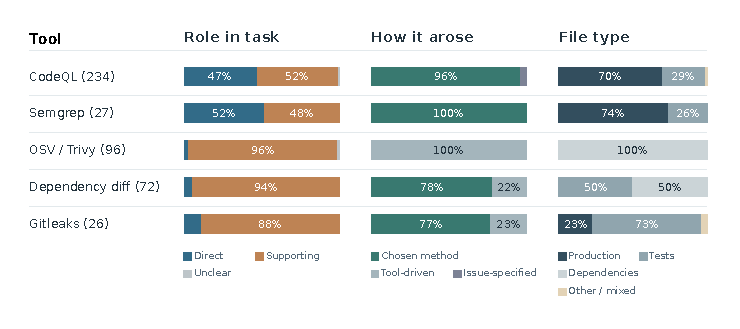
\includegraphics[width=\linewidth]{assets/figures/Fig3_Scanner.pdf}
\caption{Tool-level composition of 455 mapped changes in 191 instances. Each row uses the tool's change count as denominator, and each panel has its own legend. Task-role colours denote Direct, Supporting and Unclear. The other panels show the original implementation-origin and file-type labels. These change-level labels are distinct from the 342-choice classification in Table~\ref{tab:routes}, and the version behind the origin panel is uncertain. The file-type panel retains the known dot-ai README misclassification discussed in Section~\ref{sec:s3}; it is not a corrected estimate of production exposure. All original bars and percentages are restored without recalculation.}
\Description{Three original panels show task role, implementation-origin labels and file type by reporting tool, with separate complete legends. The original values are preserved; the caption identifies the historical classification limits and the known README file-type error.}
\label{fig:scanner}
\end{figure}

\begin{table}[H]
\caption{How 342 implementation choices were classified using public evidence (455 responsible changes, 191 instances).}
\label{tab:routes}
\small
\begin{tabular}{@{}lrrrr@{}}
\toprule
\textbf{Version} & \textbf{H} & \textbf{T} & \textbf{M} & \textbf{U}\\
\midrule
Primary frozen classification & 6 & 103 & 233 & 0\\
Earlier classification snapshot & 5 & 103 & 234 & 0\\
\bottomrule
\end{tabular}
\par\smallskip\raggedright\footnotesize Among the 233 choices classified as selected among alternatives, 77 have a specific precursor, precedent or contract (T1--T3), 128 have contextual support alone (T4), four have no independently identified public explanation (T5), and 24 have critical evidence missing (Incomplete). These are the final model-assisted classifications. The preceding classification version differed for 43 implementation choices; it is shown to expose version sensitivity, not pooled into the primary analysis. Independent blind human agreement on these labels is unavailable. Similar aggregate totals do not imply stable individual classifications. ``Incomplete'' concerns the explanation tier, whereas U concerns the broader H/T/M classification; incomplete evidence for an earlier precedent does not automatically make that broader category unresolved. Zero U labels therefore does not establish complete certainty.
\end{table}

\suppbox{Additional patterns from archived records}{%
\renewcommand{\arraystretch}{1.12}%
\begin{tabularx}{\linewidth}{@{}L{3.2cm}Y@{}}
\texttt{js/insecure-\allowbreak temporary-\allowbreak file} & 44 responsible changes in 18 repositories; 26 are test-only Supporting changes.\\
\texttt{js/file-\allowbreak system-\allowbreak race} & 17 responsible changes in 13 repositories. One responsible change can be associated with multiple rules.\\
\textbf{Tool-generated choices} & At least one choice classified as mechanical appeared in 13/20 dependency-maintenance or compatibility/migration instances, versus 2/38 feature instances in the initial subset.\\
\end{tabularx}}

% =====================================================================
\FloatBarrier
\section{RQ2 Matching and Sensitivity}\label{sec:s5}

\suppbox{Matched-control procedure (RQ2)}{%
\renewcommand{\arraystretch}{1.12}%
\begin{tabularx}{\linewidth}{@{}L{0.8cm}Y@{}}
\textbf{01} & Identify eligible candidate controls. Same-repository candidates must cover the positive's completed checks; cross-repository candidates must have exactly the same set of completed checks.\\
\textbf{02} & Apply the frozen date and change-size calipers (Section~\ref{sec:rq2-design}); exclude ineligible candidate pairs.\\
\textbf{03} & Solve one-to-one matching without replacement, prioritising maximum pair count, then same-repository pairs, then minimum normalised date/size distance, in that order.\\
\textbf{04} & Freeze the pair map; only then join the issue-wording annotations. No pair-specific re-annotation. Figure~\ref{fig:rq2-method} shows the matching stages.\\
\end{tabularx}}

\suppbox{Issue-wording codes and inference boundary}{%
\renewcommand{\arraystretch}{1.12}%
\begin{tabularx}{\linewidth}{@{}L{2.3cm}Y@{}}
\textbf{Problem only} & Problem or goal without a proposed implementation.\\
\textbf{Suggests solution} & Approach proposed, without fixing the method.\\
\textbf{Explicit instruction} & A concrete implementation instruction; distinct from H (exact mechanism prescribed).\\
\textbf{Statistical test} & Paired $3\times3$ Stuart--Maxwell test with matched pairs as units; categories are not a numeric score. Explicit-versus-other proportions are descriptive.\\
\textbf{Multiple tests} & Holm correction covered nine comparisons. These assessed issue purpose, instruction specificity, issue--PR goal alignment, implementation category, formal human review, issue-to-PR delay, shared issue/PR authorship, prior requester activity, and coding-agent or tool identity.\\
\textbf{Interpretation} & Issue-wording specificity is not a measurement of security requirements or the precise risky mechanism.\\
\end{tabularx}}

\begin{figure}[H]
\centering
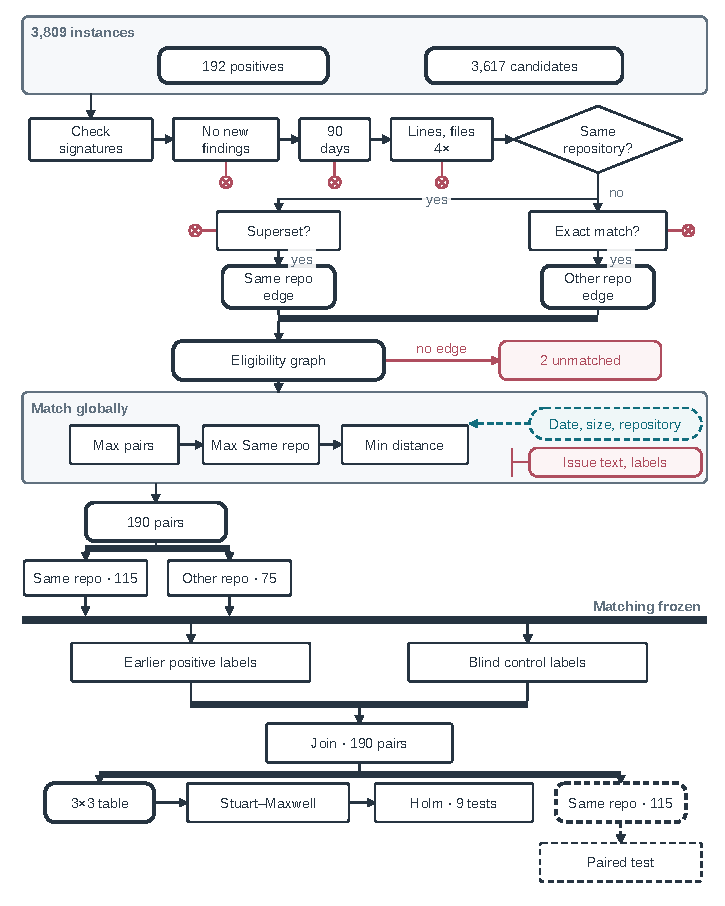
\includegraphics[width=0.85\textwidth]{assets/figures/RQ2_Methodology.pdf}
\caption{RQ2 matched comparison, showing eligibility checks and one-to-one matching. Labels were joined to pairs only after matching was frozen. Red end markers indicate failed eligibility checks; the dashed branch shows the nested same-repository sensitivity analysis.}
\Description{Finding-positive instances and candidate controls are filtered by completed checks, date and change size. Global matching prioritises pair count and same-repository pairs before issue labels are joined.}
\label{fig:rq2-method}
\end{figure}

\begin{table}[H]
\caption{RQ2 matching diagnostics, subsets and secondary comparisons. Values come from archived analysis unless identified as recomputed.}
\label{tab:rq2-diag}
\footnotesize\renewcommand{\arraystretch}{1.12}
\begin{tabularx}{\linewidth}{@{}L{5.0cm}Y@{}}
\toprule
\textbf{Quantity} & \textbf{Value}\\
\midrule
\multicolumn{2}{@{}l}{\textit{Matching}}\\
Positives matched & 190 of 192 (115 same-repository, 75 cross-repository); two without an eligible control\\
Calipers & 90 days PR date; about fourfold changed lines and files\\
Median absolute date separation & 6.66 days\\
Median larger-to-smaller ratio & 1.26 changed lines; 1.22 changed files\\
\multicolumn{2}{@{}l}{\textit{Wording, all 190 pairs (Table~\ref{tab:rq2})}}\\
Explicit instruction & 121 positives vs 148 controls ($-14.2$ points)\\
Discordant pairs & Explicit 23 positive-only vs 50 control-only; Suggests solution 33 vs 9; Problem only 26 vs 23 (recomputed from Table~\ref{tab:rq2})\\
\multicolumn{2}{@{}l}{\textit{Subsets (nested, not independent)}}\\
Original-cohort pairs & 73 of 121 vs 93 of 121 explicit ($-16.5$ points)\\
Same-repository pairs & 77 of 115 vs 95 of 115 explicit; paired $p=0.00645$\\
Direct-only positive instances & 48 of 78 vs 58 of 78 explicit\\
Supporting-only positive instances & 60 of 94 vs 75 of 94 explicit\\
Mixed positive instances & 13 of 15 on both sides; three pairs unassigned\\
\multicolumn{2}{@{}l}{\textit{Secondary comparison}}\\
Issue--PR goal alignment & 160 of 190 vs 183 of 190; $p=0.00102$, $p_{\mathrm{Holm}}=0.00815$; within repositories $p\approx0.077$\\
\bottomrule
\end{tabularx}
\end{table}

\begin{figure}[H]
\centering
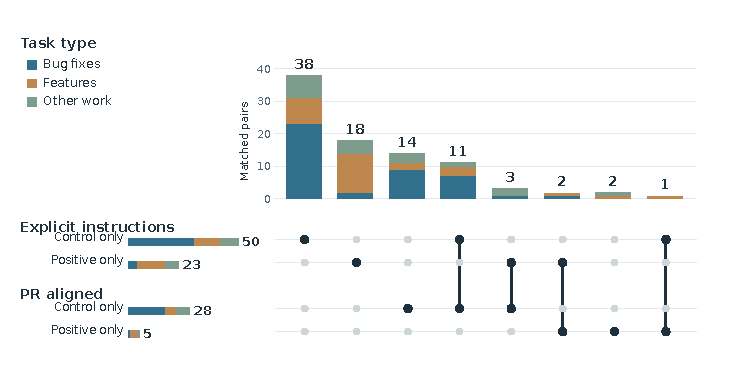
\includegraphics[width=0.85\linewidth]{assets/figures/Fig4_RQ2.pdf}
\caption{RQ2 paired differences in issue explicitness and PR goal alignment, by task type of the finding-positive issue. Bars show the 89 of 190 pairs that differ on at least one measure; the other 101 have the same status on both sides. Descriptive, not causal.}
\Description{The figure displays paired differences in explicit implementation instructions and issue to PR goal alignment for 89 discordant matched pairs, grouped by task type. The other 101 pairs have matching status on both measures.}
\label{fig:rq2-results}
\end{figure}

% =====================================================================

\FloatBarrier
\section{RQ3 Replay Evidence}\label{sec:s6}

\begin{table}[H]
\caption{Inputs for the retrospective O/W/P comparison. W and P use information from the historical warning; they do not test whether equivalent guidance could be identified prospectively.}
\label{tab:m2}
\footnotesize\renewcommand{\arraystretch}{1.12}
\begin{tabularx}{\linewidth}{@{}L{1.5cm}YY@{}}
\toprule
\textbf{Condition} & \textbf{Information supplied} & \textbf{Interpretation}\\
\midrule
\textbf{O} & Original public issue alone. & Baseline reimplementation.\\
\textbf{W} & Issue plus its historical CodeQL warning. & Retrospective warning information.\\
\textbf{P} & Issue plus a warning-derived security property, without naming the rule. & Retrospective property information.\\
\bottomrule
\end{tabularx}
\end{table}

\begin{figure}[H]
\centering
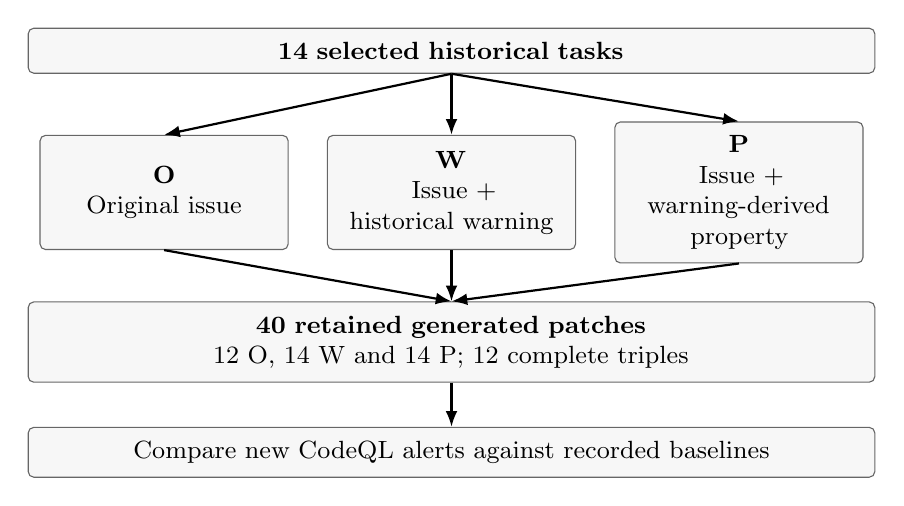
\begin{tikzpicture}[
font=\small,>={Latex[length=2mm]},
box/.style={draw=black!60,fill=black!3,rounded corners=2pt,align=center,inner sep=5pt},
wide/.style={box,text width=10.4cm},
arm/.style={box,text width=2.8cm,minimum height=1.45cm},
link/.style={->,line width=.8pt}]
\node[wide] (tasks) at (0,0) {\textbf{14 selected historical tasks}};
\node[arm] (o) at (-3.65,-1.8) {\textbf{O}\\Original issue};
\node[arm] (w) at (0,-1.8) {\textbf{W}\\Issue +\\historical warning};
\node[arm] (p) at (3.65,-1.8) {\textbf{P}\\Issue +\\warning-derived property};
\node[wide] (outputs) at (0,-3.7) {\textbf{40 retained generated patches}\\12 O, 14 W and 14 P; 12 complete triples};
\node[wide] (scans) at (0,-5.1) {Compare new CodeQL alerts against recorded baselines};
\draw[link] (tasks.south) -- (o.north);
\draw[link] (tasks.south) -- (w.north);
\draw[link] (tasks.south) -- (p.north);
\draw[link] (o.south) -- (outputs.north);
\draw[link] (w.south) -- (outputs.north);
\draw[link] (p.south) -- (outputs.north);
\draw[link] (outputs) -- (scans);
\end{tikzpicture}
\caption{The O/W/P replay comparison. Each available task-condition combination has one retained output. Independent generation sessions and functional equivalence were not verified, and missing O outputs are not counted as zero.}
\Description{Fourteen historical tasks receive original-issue, warning or property inputs. Forty outputs include twelve complete triples, whose new CodeQL alerts are compared with recorded baselines.}
\label{fig:rq3-method}
\end{figure}

\subsection*{Replay records and excluded pilot}

Section~\ref{sec:rq3-design} describes task selection and the available output-to-scan links. The syntax check covers O/W/P outputs only. The OpenAgents original-issue output (case 16633-O) recorded zero new alerts but failed that check; the check does not establish functional task completion.

A separate P1--P5 guidance pilot is excluded from these comparisons. The available records do not establish whether its summary corresponds to the intended rerun, whether the stages were independent model generations, or which pinned baseline and head scans support every result. Some outputs or intermediate records are also missing. The complete original protocol descriptions, reported counts and qualifications are preserved separately in the source package; they are not evidence of a guidance effect here.

\suppbox{Replay-case coverage}{The following six cases supplement cc-wf-studio (main text, Case~4) for the O/W/P comparison in Table~\ref{tab:replays}. Other tasks with complete triples are oh-my-claudecode \#257, opencodex \#1048, Remotion \#10147, OpenAgents \#8637 and Veritas Kanban \#906. Original-issue outputs are missing for Lepton \#226 and Trilium \#7571.}

\begin{casefile}{\textbf{Ruler symlink-safe writes}\ \ {\scriptsize\texttt{intellectronica/\allowbreak ruler}}\ \ {\scriptsize Case 3429}}{\href{https://github.com/intellectronica/ruler/issues/570}{Issue \#570}\ \ \href{https://github.com/intellectronica/ruler/pull/571}{PR \#571}\ \ \href{https://github.com/intellectronica/ruler/blob/e6eeac67de8a5afd2f00223926c156c989436482/src/agents/CrushAgent.ts}{CrushAgent.ts}}
\crow{Request}{Generated writes must not follow a symlink at the final output path, including when backups are disabled (Explicit instruction).}
\crow{Historical PR}{Replaces direct writes with \texttt{writeGeneratedFile}, which already checks for symlinks.}
\crow{Warning}{CodeQL \texttt{js/insecure-temporary-file} at \texttt{FileSystemUtils.ts}:345, a statement already in the base commit. Mapped through the flow step \texttt{CrushAgent.ts}:84 (Direct).}
\crow{Replay}{O and W each recorded one new alert; P recorded zero.}
\crow{Limit}{Zero-alert outputs are not shown to implement the task or to repair the warning site, which predates the PR.}
\end{casefile}

\begin{casefile}{\textbf{Grok CLI Telegram voice input}\ \ {\scriptsize\texttt{superagent-ai/\allowbreak grok-cli}}\ \ {\scriptsize Case 8152}}{\href{https://github.com/superagent-ai/grok-cli/issues/208}{Issue \#208}\ \ \href{https://github.com/superagent-ai/grok-cli/pull/210}{PR \#210}\ \ \href{https://github.com/superagent-ai/grok-cli/blob/80fc7fbdedacc072e9ee7eb7ac8e9a1e66d493b0/src/telegram/audio-input.ts}{audio-input.ts}}
\crow{Request}{Support voice input through Telegram (Problem only).}
\crow{Historical PR}{Fetches media from \texttt{api.telegram.org/\allowbreak file/\allowbreak bot\ldots/\allowbreak\{file\_path\}}, creates a temporary directory with \texttt{mkdtemp}, writes the downloaded audio file with mode \texttt{0600}, transcribes it, and removes the temporary directory.}
\crow{Warning}{CodeQL \texttt{js/file-access-to-http} (line 71) and \texttt{js/http-to-file-access} (line 79). Both Direct, on PR-added lines.}
\crow{Replay}{The O/W/P records contain two, one and two new alerts, respectively.}
\crow{Limit}{The reports concern network/file flows in voice processing. This is a different task from the Grok CLI file-mentions case.}
\end{casefile}

\begin{casefile}{\textbf{Open Design key storage}\ \ {\scriptsize\texttt{nexu-io/\allowbreak open-design}}\ \ {\scriptsize Case 12344}}{\href{https://github.com/nexu-io/open-design/issues/6330}{Issue \#6330}\ \ \href{https://github.com/nexu-io/open-design/pull/6356}{PR \#6356}\ \ \href{https://github.com/nexu-io/open-design/blob/b65a8b009ed95669337c8a193130a81471ecd44a/apps/daemon/src/routes/runs.ts}{runs.ts}}
\crow{Request}{Persist BYOK keys reliably on Windows and fail clearly instead of silently falling back to cloud billing (Suggests solution).}
\crow{Historical PR}{The PR rolls back the secure credential-profile design to browser-local BYOK configuration. The mapped change is a configuration-completeness check in \texttt{routes/runs.ts}:849.}
\crow{Warning}{CodeQL \texttt{js/remote-property-injection} and \texttt{js/polynomial-redos} at \texttt{byok-opencode.ts}:80 and :104, statements present before the PR. One Direct change, mapped through a flow location.}
\crow{Replay}{None of the three O/W/P outputs recorded an alert under either historical rule; their recorded alerts concern other rules.}
\crow{Limit}{Absence of the historical rules did not mean an alert-free output; the recorded alerts concern other rules.}
\end{casefile}

\begin{casefile}{\textbf{Oracle downloadable artifacts}\ \ {\scriptsize\texttt{steipete/\allowbreak oracle}}}{\href{https://github.com/steipete/oracle/issues/244}{Issue \#244}\ \ \href{https://github.com/steipete/oracle/pull/245}{PR \#245}\ \ \href{https://github.com/steipete/oracle/blob/ac32c892437ad4b92f0e1ddb5d9e90ad195e38a9/src/browser/artifacts.ts}{artifacts.ts}}
\crow{Request}{Save browser-generated downloadable artifacts rather than only linking them in a transcript.}
\crow{Historical PR}{Writes downloaded bytes using \texttt{writeBinaryBrowserArtifact}, which sanitises the filename and checks for an unused target path before writing.}
\crow{Warning}{CodeQL \texttt{js/http-to-file-access}. Extended provenance records contain a mapping, not independently revalidated for this case card; this task is outside the original 122-instance workbook.}
\crow{Replay}{The historical rule was recorded under all three O/W/P conditions.}
\crow{Limit}{Functional equivalence and any repair are not established.}
\end{casefile}

\begin{casefile}{\textbf{Neo.mjs Fleet service}\ \ {\scriptsize\texttt{neomjs/\allowbreak neo}}}{\href{https://github.com/neomjs/neo/issues/16735}{Issue \#16735}\ \ \href{https://github.com/neomjs/neo/pull/16761}{PR \#16761}\ \ \href{https://github.com/neomjs/neo/blob/6bf4ebc2d4acaea88faf293cd7e670fe9e3fd4ec/ai/scripts/diagnostics/fleetHealthcheck.mjs}{fleetHealthcheck.mjs}}
\crow{Request}{An optional authenticated Fleet server and healthcheck probe with file-sourced bearer credentials.}
\crow{Historical PR}{The probe reads a bearer token from a configured file and sends it to a configurable URL (default loopback, with a timeout).}
\crow{Warning}{CodeQL \texttt{js/file-access-to-http}, \texttt{fleetHealthcheck.mjs}:107. An extended-provenance mapping is archived but not independently revalidated here; this task is outside the original 122-instance workbook.}
\crow{Replay}{The property condition matched the original-issue condition in recorded alert counts.}
\crow{Limit}{The zero-alert W output may omit functionality. This is a different task from the Neo.mjs wake receiver.}
\end{casefile}

\begin{casefile}{\textbf{Delegate Skills Windows relay}\ \ {\scriptsize\texttt{amElnagdy/\allowbreak delegate-skills}}}{\href{https://github.com/amElnagdy/delegate-skills/issues/3}{Issue \#3}\ \ \href{https://github.com/amElnagdy/delegate-skills/pull/13}{PR \#13}\ \ \href{https://github.com/amElnagdy/delegate-skills/blob/2c8d988f0d9542f7c005d8cf7f709005a63d1ba3/skills/grok-delegate/scripts/relay.mjs}{relay.mjs}}
\crow{Request}{Fix Windows quoting and path failures in an existing codex-delegate relay.}
\crow{Historical PR}{A new Grok relay writes brief, event and result files beneath an \texttt{os.tmpdir()} path named from repository and timestamp, created recursively rather than with \texttt{mkdtemp}.}
\crow{Warning}{Four CodeQL \texttt{js/insecure-temporary-file} locations in \texttt{relay.mjs}. An extended-provenance mapping is archived but not independently revalidated here; this task is outside the original 122-instance workbook.}
\crow{Limit}{The linked issue and PR differ in scope, limiting what a reimplementation of the issue can test.}
\end{casefile}


\clearpage

\includepdf[pages=-,fitpaper=true,pagecommand={\thispagestyle{empty}}]{assets/declaration/AI_declaration_signed.pdf}
\end{document}
